\documentclass[11pt,a4paper]{article}
\usepackage[utf8]{inputenc}
\usepackage[T1]{fontenc}
\usepackage[brazil]{babel}
\usepackage[margin=2.5cm]{geometry}
\usepackage{booktabs}
\usepackage{amsmath,amssymb}
\usepackage{caption}
\usepackage{graphicx}
\usepackage{setspace}
\usepackage{enumitem}
\usepackage{placeins}
\usepackage{longtable}
\usepackage{float}
\usepackage[hidelinks]{hyperref}
\graphicspath{{v2 OFICIAL/figuras/}}
\setstretch{1.4}
\captionsetup{font=small,labelsep=colon}
\setcounter{tocdepth}{2}

\title{Peso de VALE3 nos fundos de investimento brasileiros:\\
um modelo de fator dinâmico com correção logística e ajuste parcial}
\author{João Paulo Zangrandi\\
Fundação Getulio Vargas --- Escola de Economia de São Paulo (FGV--EESP)\\
Orientador: Prof.\ Mauricio Ferraresi}
\date{}

\begin{document}
\maketitle

\tableofcontents
\newpage

% ======================================================================
\section{Introdução}

\emph{[Seção a ser escrita por último.]}

% ======================================================================
\section{Revisão de literatura}

\emph{[Seção a ser desenvolvida após indicação de referências pelo orientador. Áreas de
inserção previstas: precificação de ativos baseada em demanda (\emph{demand-based asset
pricing}); comportamento de fundos de investimento e efeitos de fluxo; modelos de ajuste
parcial em finanças corporativas e de portfólio.]}

% ======================================================================
\section{Dados}
\label{sec:dados}

\FloatBarrier
\subsection{Fontes}

Os dados usados neste trabalho vêm de dois registros públicos que a Comissão de Valores
Mobiliários (CVM) exige de todo fundo de investimento brasileiro. O primeiro é a Composição e
Diversificação de Aplicações (CDA), um extrato mensal em que cada fundo declara, ativo por
ativo, o valor de mercado e a participação percentual de cada posição em sua carteira --- é
dele que vem a variável dependente deste trabalho, o peso de um ativo na carteira de um fundo
em um determinado mês. O segundo é o Informe Diário, que traz, para cada fundo e cada dia útil,
o patrimônio líquido, o número de cotistas, a captação e o resgate do dia, e o valor da cota
--- é dele que vêm as características do fundo usadas como variáveis explicativas.

\FloatBarrier
\subsection{Universo e período}

O período coberto vai de janeiro de 2016 a dezembro de 2021. O universo de fundos partiu dos
fundos administrados pelo grupo Itaú e foi ampliado, em etapas, para tornar os resultados mais
gerais e menos sujeitos a alguma particularidade de uma única gestora. A ampliação seguiu dois
eixos independentes: o primeiro amplia \emph{quais fundos} entram na amostra --- de só Itaú
(308 fundos) para todo o universo CVM que já teve VALE3 em carteira em algum momento do período
(2.820 fundos, agrupados em 41 grupos de gestora por marca controladora; por exemplo, os quatro
rótulos que a CVM usa para a BTG Pactual são tratados como um único grupo); o segundo amplia
\emph{quais ativos} são observados dentro desses mesmos fundos --- de um único papel (VALE3)
para todas as ações que eles carregam.

Cada etapa dessa ampliação produz \textbf{dois} números de fundos, que não devem ser confundidos
entre si. O \textbf{universo bruto} é quantos fundos entram na consideração, só pelo critério de
elegibilidade (ser do grupo Itaú, ou já ter tido VALE3 em algum momento) --- não depende de
nenhum dado além da posição em si. A \textbf{amostra final} é quantos desses fundos sobram depois
de exigidas as cinco características do modelo (Seção~\ref{sec:metodologia}) simultaneamente
disponíveis em pelo menos um mês --- um número sempre menor que o universo bruto, porque nem todo
fundo tem AUM, cotistas, fluxo, indicador de FIC e beta completos ao mesmo tempo em algum mês. A
Tabela~\ref{tab:universo} mostra as duas colunas lado a lado.

\begin{table}[h]\centering\small
\caption{Evolução do universo de dados ao longo do trabalho.}
\label{tab:universo}
\begin{tabular}{@{}p{6.0cm}rrrrr@{}}
\toprule
 & \multicolumn{2}{c}{Fundos} & & & \\
Etapa & Universo & Amostra final & Gestoras & Ativos & Observações \\
\midrule
Amostra inicial (só Itaú, só VALE3) & 308 & 250 & 1 & 1 & 8.335 \\
Ampliação de gestoras (todo o universo CVM, só VALE3) & 2.820 & 2.295 & 41 & 1 & 71.569 \\
Ampliação de ativos (todo o universo CVM, todas as ações) & 2.820 & 2.347 & 41 & 501 & 8.268.920 \\
\bottomrule
\end{tabular}
\caption*{\footnotesize Observações em fundo(-ativo)-mês. A Seção~\ref{sec:resultados} organiza
os resultados por etapa (Seção~\ref{sec:metodologia}): as Etapas 1 e 2 (estimativas e erros $e$,
$u$) usam a amostra inicial (250 fundos, só VALE3); a Etapa 3 (erro fora da amostra) começa nessa
mesma amostra inicial e depois generaliza para a amostra amplamente expandida (última linha desta
tabela).}
\end{table}

Um detalhe da Tabela~\ref{tab:universo} merece atenção porque, à primeira vista, parece
contraditório: a coluna de amostra final \textbf{cresce} da segunda para a terceira linha (de
2.295 para 2.347 fundos) mesmo com o universo bruto permanecendo \textbf{idêntico} (2.820 nos
dois casos --- é literalmente o mesmo conjunto de fundos). A explicação está em como a exigência
das cinco características é aplicada: um fundo só entra na amostra final se tiver, em
\textbf{algum} mês, todas as cinco disponíveis ao mesmo tempo. Na etapa ``só VALE3'', esse "algum
mês" só pode ser um mês em que o fundo carregava VALE3 --- se, digamos, um fundo teve VALE3 só em
janeiro e fevereiro de 2018, e o número de cotistas dele faltava no Informe Diário da CVM
justamente nesses dois meses, esse fundo fica de fora da amostra final, mesmo que em outros meses
(sem VALE3) ele tivesse as cinco características completas. Na etapa ``todas as ações'', esse
mesmo fundo ganha uma chance a mais: se ele carregava, por exemplo, Petrobras em março de 2018, e
nesse mês o dado de cotistas estava completo, esse mês passa a contar, e o fundo entra na amostra
final --- sem que nenhum fundo novo tenha sido adicionado ao universo bruto. Olhar todas as ações
que um fundo carrega, em vez de só VALE3, multiplica o número de (fundo, mês) candidatos a
satisfazer as cinco exigências de dado ao mesmo tempo; por isso a amostra final cresce, mesmo
partindo do mesmo universo de 2.820 fundos.

Vale perguntar, especificamente, por que 473 dos 2.820 fundos do universo bruto (todas as
gestoras, todos os ativos, sem nenhum filtro por ativo específico) ficam de fora da amostra
final. A resposta, verificada fundo a fundo sobre o histórico completo de cotas de 2016 a 2021
(não uma amostra): 28 fundos (5,9\% dos 473) nunca têm patrimônio, cotistas, fluxo e indicador
de FIC completos ao mesmo tempo em nenhum mês, independente do beta. Os outros 445 (94,1\%) têm
essas quatro características completas em algum mês, mas nunca chegam a ter beta --- e o motivo,
para a esmagadora maioria deles, é simplesmente não ter acumulado histórico de cota suficiente
dentro da janela do trabalho, não fechamento precoce: 406 desses 445 fundos (91,2\%) nunca somam
252 dias de cota válida em toda a janela 2016--2021, e portanto jamais teriam beta calculável
mesmo que a amostra usasse o período inteiro; dentre estes, 263 (65\%) só começam a reportar
cota em 2021, isto é, são fundos jovens demais para acumular um ano de histórico antes do fim da
amostra (dezembro de 2021). Um grupo bem menor, 18 fundos (4,0\% dos 445), tem os 252 dias
acumulados sem lacunas relevantes na série, mas começa a reportar cota por volta de
novembro/dezembro de 2020 --- tarde o suficiente para que o primeiro beta válido só surgisse
perto do fim da amostra, sem mais nenhum mês seguinte disponível para usá-lo como preditor
defasado (t$-$1). Apenas os 21 fundos restantes (4,7\% dos 445) têm histórico suficiente que
termina antes de novembro de 2021, um padrão mais consistente com fechamento ou saída do fundo.
Em suma: quase toda a perda de fundos por causa do beta (424 dos 445, ou 95,3\%) reflete fundos
jovens demais para a janela do trabalho, não uma limitação de dado nem fundos que encerraram
atividades.

A mesma exigência simultânea das cinco características do fundo (Seção~\ref{sec:metodologia})
também reduz a cobertura temporal de 72 para 59 meses efetivos (fevereiro de 2017 a dezembro de
2021): o beta do fundo precisa de pelo menos 252 pregões de histórico de cota (cerca de um ano)
para ser calculado, o que deixa os primeiros doze meses da amostra sem fundos suficientes. Essa
perda de cobertura inicial foi uma escolha deliberada, não uma limitação inesperada do dado:
preferiu-se um conjunto menor de meses com as cinco características completas a um conjunto
maior com características faltantes preenchidas de forma arbitrária.

\FloatBarrier
\subsection{Limpeza de custódia}

Um mesmo ativo pode aparecer na CDA sob rótulos diferentes conforme o tipo de posição que o
fundo mantém: posição direta, posição cedida ou recebida em empréstimo, ou direito de
subscrição. Manter todos esses rótulos juntos infla artificialmente o peso de um ativo e mistura
posições de natureza econômica distinta. Este trabalho mantém apenas a posição direta,
identificada pelo sufixo numérico do código de negociação (convenção da B3: os sufixos 3, 4, 5,
6, 7, 8 e 11 correspondem a ações ordinárias, preferenciais e units; outros sufixos e palavras-chave
associadas a empréstimo ou subscrição são descartados). Essa limpeza resulta em 523 ativos de
posição direta e 10.603.928 linhas de fundo-ativo-mês antes dos demais filtros.

\FloatBarrier
\subsection{Características do fundo}

Cinco características de cada fundo entram no modelo, todas medidas no último dia do mês
anterior ao da observação --- nenhuma delas usa informação contemporânea ao próprio mês, o que
evita viés de antecipação (\emph{look-ahead bias}): o tamanho do fundo (logaritmo do
patrimônio líquido), o número de cotistas (logaritmo), um indicador de ser fundo de cotas de
outro fundo (FIC), o fluxo líquido de captação menos resgate como proporção do patrimônio, e o
beta do próprio fundo --- a covariância do retorno diário da cota do fundo com o retorno do
Ibovespa, dividida pela variância do retorno do Ibovespa, numa janela móvel de 252 pregões,
terminando no último pregão do mês anterior. As quatro primeiras características vêm do Informe
Diário; a quinta é construída a partir da série de cotas do próprio fundo.

\FloatBarrier
\subsection{Amostra final}

Depois de exigidas as cinco características simultaneamente, a amostra usada na etapa de
regressão cross-section por ativo-mês (Seção~\ref{sec:metodologia}) tem 8.268.920 observações
de fundo-ativo-mês, cobrindo os 2.347 fundos e 501 ativos mencionados. A Tabela~\ref{tab:amostra}
resume as principais dimensões dessa amostra final.

\begin{table}[h]\centering
\caption{Dimensões da amostra final (base multiativo --- todas as gestoras, todos os ativos).}
\label{tab:amostra}
\begin{tabular}{@{}lr@{}}
\toprule
Observações (fundo $\times$ ativo $\times$ mês) & 8.268.920 \\
Fundos & 2.347 \\
Grupos de gestora & 41 \\
Ativos (posição direta) & 501 \\
Meses (fev/2017--dez/2021) & 59 \\
\bottomrule
\end{tabular}
\caption*{\footnotesize Esta é a maior base do trabalho, mas \textbf{não} é usada em todas as
tabelas e figuras da Seção~\ref{sec:resultados} --- só na parte generalizada da Etapa 3
(Seção~\ref{sec:resultados}.3, a partir da Figura~\ref{fig:dinamica-gestora}). As Seções~5.1, 5.2
e o início da 5.3 usam a amostra inicial menor (VALE3--Itaú, 250 fundos, Tabela~\ref{tab:universo}).
Cada tabela e figura a seguir indica explicitamente qual base usa.}
\end{table}

\emph{[Tabelas/figuras adicionais de cobertura --- por exemplo, distribuição do número de
fundos por gestora, ou evolução do número de fundos ativos por mês --- a incluir conforme
indicação do orientador na próxima reunião.]}

% ======================================================================
\section{Metodologia}
\label{sec:metodologia}

O trabalho é organizado em três etapas sequenciais, cada uma alimentando a seguinte. A primeira
etapa estima, mês a mês, o peso que cada fundo \emph{deveria} carregar em cada ativo, dadas as
características observáveis do fundo. A segunda etapa modela a velocidade com que o peso
efetivamente observado converge a esse alvo. A terceira etapa testa, em dados que o modelo nunca
viu durante a estimação, se essa modelagem tem valor preditivo genuíno. Em cada uma das três
etapas, o erro --- a diferença entre o que o modelo previu e o que de fato aconteceu --- não é
descartado: ele é o principal objeto de análise deste trabalho, na medida em que sua estrutura
(quem erra mais, quando, e em que direção) é o que permite comparar fundos e gestoras entre si e
avaliar se o modelo tem poder explicativo genuíno ou apenas se ajusta ao passado.

\FloatBarrier
\subsection{Etapa 1: cross-section}

Para cada ativo $n$ e cada mês $t$, o peso que um fundo $i$ carrega é modelado como função
logística de cinco características do fundo:
\begin{equation}
\text{peso}_{i,n,t} = g\big(x_{i,n,t}'\theta_{n,t}\big) + e_{i,n,t}, \qquad
g(z) = \frac{1}{1+e^{-z}}
\label{eq:cs}
\end{equation}
em que $x_{i,n,t}$ reúne as cinco características descritas na Seção~\ref{sec:dados}
(padronizadas, exceto o indicador de fundo de cotas) e $\theta_{n,t}$ é o vetor de coeficientes
daquele ativo naquele mês, estimado por máxima verossimilhança (regressão logística
quase-binomial). A função $g(\cdot)$ garante que a previsão nunca saia do intervalo $[0,1]$,
respeitando o fato de que peso é, por definição, uma fração da carteira --- uma regressão linear
comum não teria essa garantia. A regressão é estimada separadamente para cada célula
(ativo, mês) que tenha um número mínimo de fundos detentores, sem nenhuma etapa de agregação
temporal por cima (não é um procedimento em dois passos como Fama--MacBeth): cada
$\theta_{n,t}$ é o resultado de uma única regressão de corte transversal.

O erro dessa etapa, $e_{i,n,t} = \text{peso}_{i,n,t} - g(x_{i,n,t}'\theta_{n,t})$, mede o quanto
a posição observada de um fundo se afasta do que suas próprias características explicam,
\emph{dentro} do mesmo mês. Por construção da máxima verossimilhança, a média desse erro é
mecanicamente zero em cada célula --- não é evidência de bom ajuste, apenas uma propriedade
algébrica do estimador. O que de fato varia, e é informativo, é a \textbf{dispersão} do erro: um
fundo cujo erro é consistentemente pequeno tem posições bem explicadas pelas cinco
características observáveis; um fundo cujo erro é grande e disperso tem posições que fogem
desse padrão --- convicção própria do gestor, não captada pelas variáveis do modelo.

\FloatBarrier
\subsection{Etapa 2: ajuste parcial}

A Etapa 1 estima um alvo, $w^*_{i,n,t} = g(x_{i,n,t}'\theta_{n,t})$, mas não diz nada sobre a
\emph{dinâmica}: quão rápido a posição real de um fundo converge a esse alvo, mês a mês. A
segunda etapa modela essa dinâmica através de um mecanismo de ajuste parcial, hipótese padrão em
modelos de rebalanceamento de portfólio: a cada mês, o fundo fecha uma fração $\lambda$ da
distância entre sua posição atual e o alvo.
\begin{equation}
w_{i,n,t+1} - w_{i,n,t} = \lambda\, d_{i,n,t} + u_{i,n,t+1}, \qquad
d_{i,n,t} \equiv w^*_{i,n,t} - w_{i,n,t}
\label{eq:pa}
\end{equation}
$\lambda$ é estimado por mínimos quadrados ordinários diretos, sem intercepto, com todos os
pares de meses consecutivos agrupados (\emph{pooled}) --- um único coeficiente, a mesma
velocidade de ajuste para todo fundo e todo ativo. O erro dessa etapa, $u_{i,n,t+1}$, mede o
quanto a mudança de posição observada difere do que o ajuste parcial previu: valores de $u$
próximos de zero indicam fundos cuja movimentação segue de perto a velocidade média de ajuste
estimada; valores grandes indicam movimentos abruptos --- apostas concentradas de curto prazo
--- que o modelo, por construção, não tem como antecipar.

\FloatBarrier
\subsection{Etapa 3: esquema fora da amostra}

As duas primeiras etapas são estimadas com a amostra inteira e, por isso, não dizem se o modelo
tem valor preditivo de verdade --- um coeficiente pode explicar bem o passado e não generalizar
para dados novos. A terceira etapa testa isso diretamente, com um corte temporal único: o
parâmetro $\lambda$ (e, na generalização a seguir, $\lambda_h$ para cada horizonte $h$) é
reestimado usando \textbf{apenas} os meses de treino, anteriores a janeiro de 2020, e então
aplicado, fixo, aos meses de teste, de janeiro de 2020 em diante --- período que o modelo nunca
viu durante a estimação.
\begin{align}
\widehat w_{i,n,t+h} &= w_{i,n,t} + \widehat\lambda_{h,\text{treino}}\, d_{i,n,t}
&&\text{(ajuste parcial)} \notag\\
\widehat w_{i,n,t+h} &= w_{i,n,t} &&\text{(previsão ingênua)}
\label{eq:oos}
\end{align}
O erro fora da amostra, $\text{erro}_{i,n,t+h} = \big(w_{i,n,t+h}-w_{i,n,t}\big) -
\widehat\lambda_{h,\text{treino}}\, d_{i,n,t}$, é comparado ao erro da previsão ingênua (que
simplesmente assume que nada muda) através da raiz do erro quadrático médio (RMSE). A diferença
percentual entre os dois RMSEs --- chamada, neste trabalho, de \textbf{margem} --- responde à
pergunta que interessa de fato: o ajuste parcial estimado com dados antigos ainda ajuda a prever
dados novos, ou uma previsão ingênua seria tão boa quanto?

\paragraph{Robustez: $\lambda$ fixo vs. janela expansiva.} O corte único mantém $\lambda_h$
congelado no valor de treino durante todo o período de teste --- uma escolha deliberada de
simplicidade (Seção~\ref{sec:metodologia}), mas que levanta a dúvida óbvia: um $\lambda_h$
reestimado a cada mês, incorporando os dados de teste já observados até ali (janela expansiva,
sem nenhum vazamento --- cada $\lambda_{h,s}$ usa só pares cujo resultado já era conhecido antes
do mês $s$), previa melhor? A Tabela~\ref{tab:janela_expansiva} responde que não, de forma
consistente nas duas versões da amostra: a razão RMSE/ingênua praticamente não muda, o padrão de
quais meses o ajuste parcial vence a previsão ingênua é idêntico entre as duas versões de
$\lambda$, e --- na base multiativo, que sustenta a maior parte desta seção de Resultados --- o
ranking de dificuldade de previsão por gestora tem correlação de Spearman de $0{,}9998$ entre as
duas versões. Isso valida empiricamente a simplificação: atualizar $\lambda_h$ mês a mês não
captura nenhuma dinâmica relevante que o valor fixo, estimado uma única vez, já não capture.

\begin{table}[h]\centering\small
\caption{$\lambda$ fixo (treino único) vs. janela expansiva (reestimado mês a mês, sem
vazamento), fora da amostra, $h=1$. Colunas 3--4: razão RMSE/RMSE ingênua.}
\label{tab:janela_expansiva}
\begin{tabular}{@{}p{4.6cm}rrr@{}}
\toprule
Base & Meses de teste & $\lambda$ fixo & $\lambda$ expansiva \\
\midrule
VALE3--Itaú (250 fundos) & 23 & $0{,}9846$ & $0{,}9813$ \\
Multiativo (2.347 fundos, 501 ativos) & 23 & $0{,}9824$ & $0{,}9824$ \\
\bottomrule
\end{tabular}
\caption*{\footnotesize Em ambas as bases, o ajuste parcial vence a previsão ingênua exatamente
nos mesmos meses sob as duas versões de $\lambda$ (14 de 23 na base VALE3--Itaú; 23 de 23 na base
multiativo).}
\end{table}

\subsubsection*{Por que a análise do erro é o centro deste trabalho}

As três etapas descritas acima poderiam ser resumidas, cada uma, num único número: um
$R^2$, um $\widehat\lambda$, uma margem agregada. Mas o valor deste trabalho está em não parar
nesse resumo. Agregando o erro fora da amostra por fundo, por gestora e por ativo --- e
comparando essa agregação entre horizontes de previsão ($h=1,3,6,12$ meses) --- é possível
identificar \emph{quais} fundos e gestoras têm posições bem explicadas pelo modelo e quais têm
comportamento que foge sistematicamente dele, de forma estável ao longo do tempo e não apenas
como um acidente de uma única janela de teste. Essa estrutura de erro é a base de toda a Seção
de Resultados deste trabalho e, potencialmente, de uma aplicação prática discutida na
Seção~\ref{sec:aplicacao}.

\FloatBarrier
\subsection{Extensões}

O procedimento descrito acima --- Etapas 1 a 3 --- é aplicado primeiro à ação VALE3 dentro dos
fundos do grupo Itaú, e depois generalizado em dois eixos independentes, já descritos na
Seção~\ref{sec:dados}: para todas as gestoras do universo CVM (através de um efeito fixo de
gestora somado ao preditor linear da equação~\eqref{eq:cs}), e para todas as ações que essas
gestoras carregam (repetindo a equação~\eqref{eq:cs} célula por célula de ativo-mês, em vez de
uma única regressão para VALE3). A Etapa 3 --- o esquema fora da amostra --- é igualmente
generalizada: o índice de ativo $n$ e o horizonte $h$ passam a ser explícitos na
equação~\eqref{eq:pa}, permitindo agregar o erro fora da amostra por gestora, por ativo e por
horizonte de previsão simultaneamente.

% ======================================================================
\section{Resultados}
\label{sec:resultados}

\emph{[Texto analítico desta seção a ser escrito após nova rodada de discussão com o
orientador. Tabelas e figuras abaixo já validadas em versões anteriores do documento de
trabalho \texttt{v2 OFICIAL.tex}; as legendas foram mantidas apenas descritivas.]}

\FloatBarrier
\subsection{Etapa 1: cross-section}

Relembrando a equação~\eqref{eq:cs}, $\text{peso}_{i,n,t} = g(x'_{i,n,t}\theta_{n,t}) + e_{i,n,t}$:
para cada ativo $n$ e mês $t$, o modelo logístico estima o peso que cada fundo $i$
\emph{deveria} carregar, a partir de $x_{i,n,t}$ (as cinco características do fundo) e
$\theta_{n,t}$ (os coeficientes daquele ativo naquele mês). O erro $e_{i,n,t}$ é a distância
entre o peso observado e essa previsão: por construção da máxima verossimilhança, sua média é
mecanicamente zero em cada célula (ativo, mês) --- não é evidência de bom ajuste, é uma
propriedade algébrica do estimador. O que de fato varia, e é informativo, é a \textbf{dispersão}
do erro: um fundo cujo erro é consistentemente pequeno tem posições bem explicadas pelas cinco
características observáveis; um fundo cujo erro é grande e disperso tem posições que fogem
desse padrão. As tabelas e figuras abaixo cobrem primeiro as estimativas de $\theta_{n,t}$, e em
seguida a estatística do erro $e$ que elas produzem.

\begin{table}[h]\centering\small
\caption{$\Theta$ logístico: antes e depois do beta do fundo (mesma amostra, 59 meses, teste
de significância $t=\bar\theta/(\text{dp}(\theta)/\sqrt{59})$). Base: VALE3--Itaú (250 fundos,
1 ativo).}
\label{tab:theta}
\begin{tabular}{@{}lrcrc@{}}
\toprule
Variável & Média (sem $\beta^{fundo}$) & Sig. & Média (com $\beta^{fundo}$) & Sig. \\
\midrule
$\alpha$                   & $-3{,}1262$ & *** & $-3{,}8110$ & *** \\
$\theta^{aum}$ (tamanho)        & $-0{,}2749$ & *** & $-0{,}0594$ & *** \\
$\theta^{cot}$ (cotistas)       & $0{,}4429$  & *** & $0{,}0493$  & *** \\
$\theta^{fic}$ (fundo de cotas) & $-0{,}6669$ & *** & $-0{,}2149$ & *** \\
$\theta^{flow}$ (captação/resgate) & $0{,}4402$ & n.s. & $0{,}1396$ & n.s. \\
$\theta^{bf}$ (beta do fundo)   & ---          & ---& $1{,}0110$  & *** \\
\midrule
Pseudo-$R^2$ (McFadden) médio & $0{,}164$ & & $0{,}614$ & \\
\bottomrule
\end{tabular}
\caption*{\footnotesize $^{*}p<5\%$, $^{**}p<1\%$, $^{***}p<0{,}1\%$.}
\end{table}

\begin{table}[h]\centering\small
\caption{Efeito marginal médio (APE) do logit, em pontos percentuais de peso --- mesma
comparação sem/com beta do fundo. Base: VALE3--Itaú (250 fundos, 1 ativo).}
\begin{tabular}{@{}lrcrc@{}}
\toprule
Característica & APE (sem $\beta^{fundo}$) & Sig. & APE (com $\beta^{fundo}$) & Sig. \\
\midrule
Tamanho              & $-0{,}00734$ & *** & $-0{,}00154$ & *** \\
Cotistas             & $0{,}01271$  & *** & $0{,}00111$  & *** \\
Fundo de cotas       & $-0{,}02222$ & *** & $-0{,}00580$ & *** \\
Captação/resgate     & $0{,}01068$  & n.s. & $0{,}00449$ & n.s. \\
Beta do fundo        & ---           & --- & $0{,}02942$  & *** \\
\bottomrule
\end{tabular}
\end{table}

\begin{figure}[h]\centering
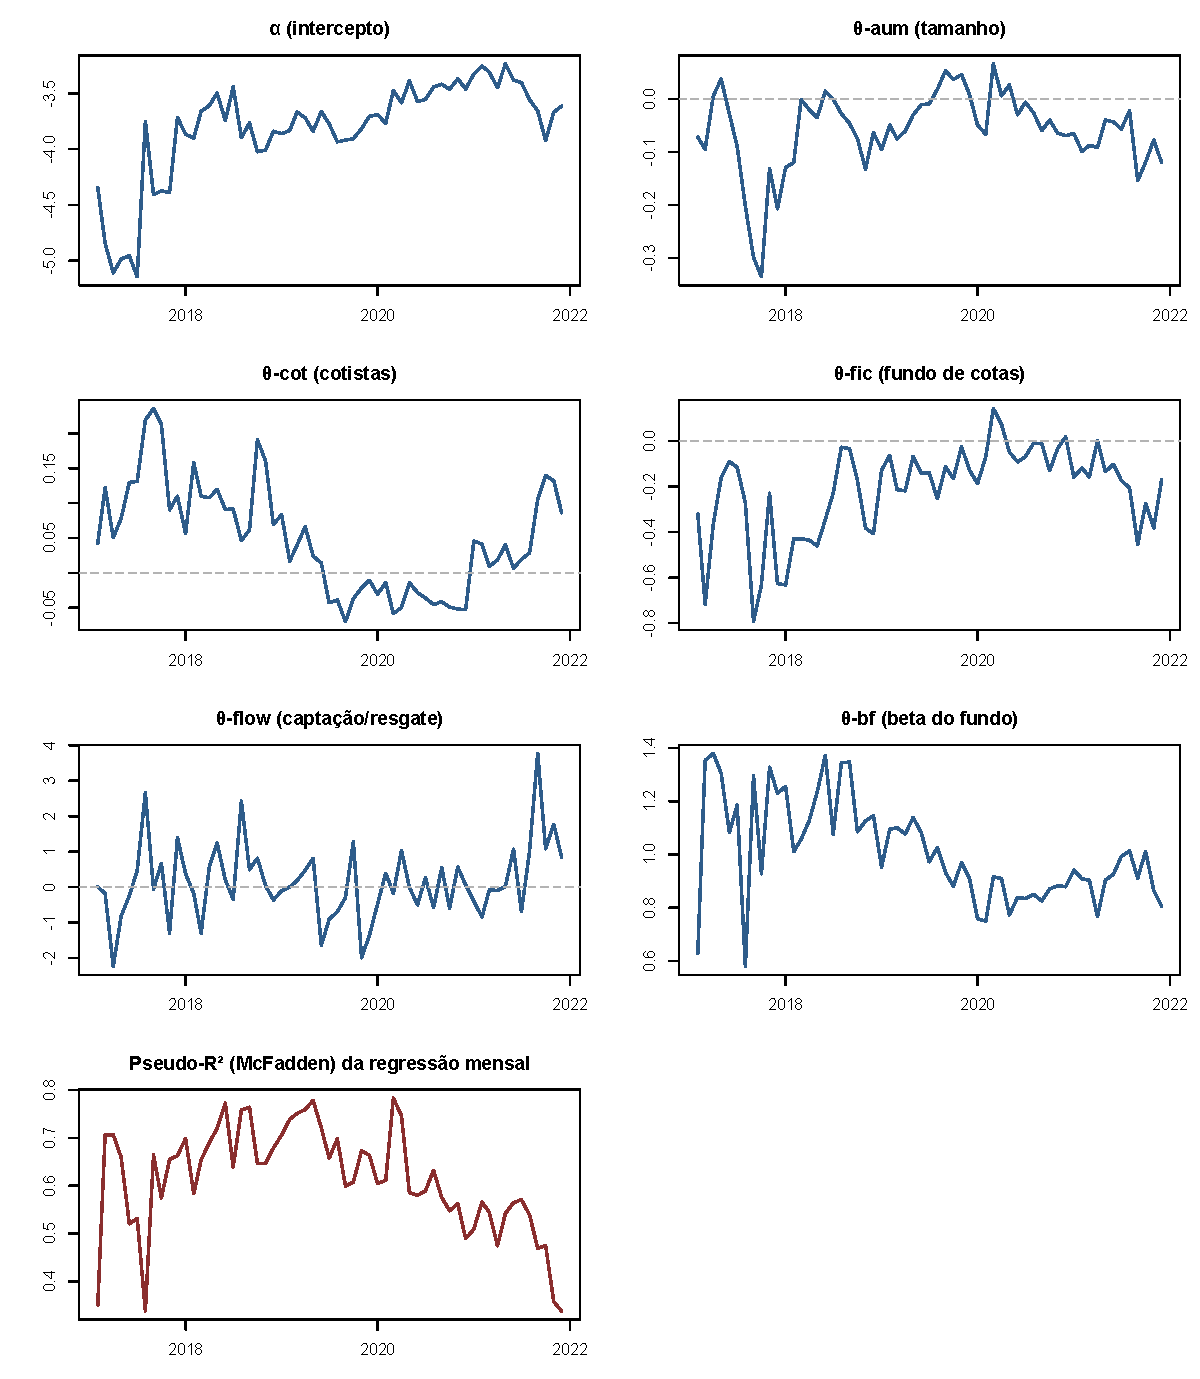
\includegraphics[width=0.75\textwidth]{fig_theta_trajetoria_v2.pdf}
\caption{Os seis componentes de $\theta_t$ logístico (com beta do fundo) ao longo dos 59 meses, e
o pseudo-$R^2$ de McFadden de cada regressão mensal. Base: VALE3--Itaú (250 fundos, 1 ativo).}
\end{figure}

\begin{table}[h]\centering\small
\caption{Estatísticas do erro $e$, Etapa 1 (8.335 observações). Base: VALE3--Itaú (250 fundos,
1 ativo).}
\begin{tabular}{@{}lr@{}}
\toprule
Estatística & Valor \\
\midrule
Média & $0{,}000000$ \\
Desvio-padrão & $0{,}0227$ \\
Mediana & $-0{,}0008$ \\
Mínimo / Máximo & $-0{,}113$ / $0{,}178$ \\
\% de observações com $e>0$ & $45{,}1\%$ \\
Assimetria & $0{,}39$ \\
Curtose & $7{,}67$ (normal $=3$) \\
Previsões fora de $[0,1]$ & $0$ de $8.335$ \\
\bottomrule
\end{tabular}
\end{table}

\begin{figure}[h]\centering
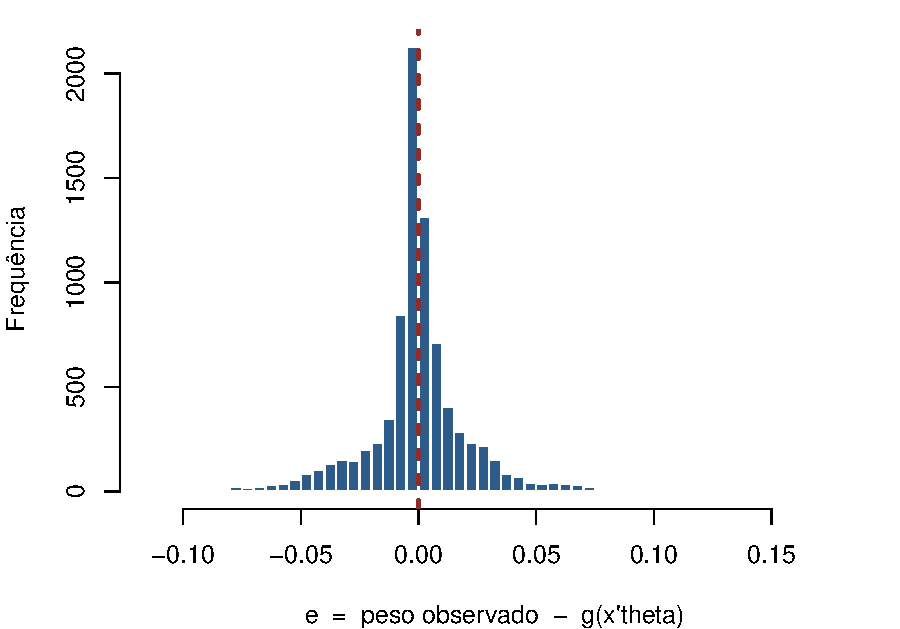
\includegraphics[width=0.65\textwidth]{hist_erro_e_v2.pdf}
\caption{Histograma do erro $e$ (8.335 observações). A linha tracejada marca zero. Base:
VALE3--Itaú (250 fundos, 1 ativo).}
\end{figure}

\begin{figure}[h]\centering
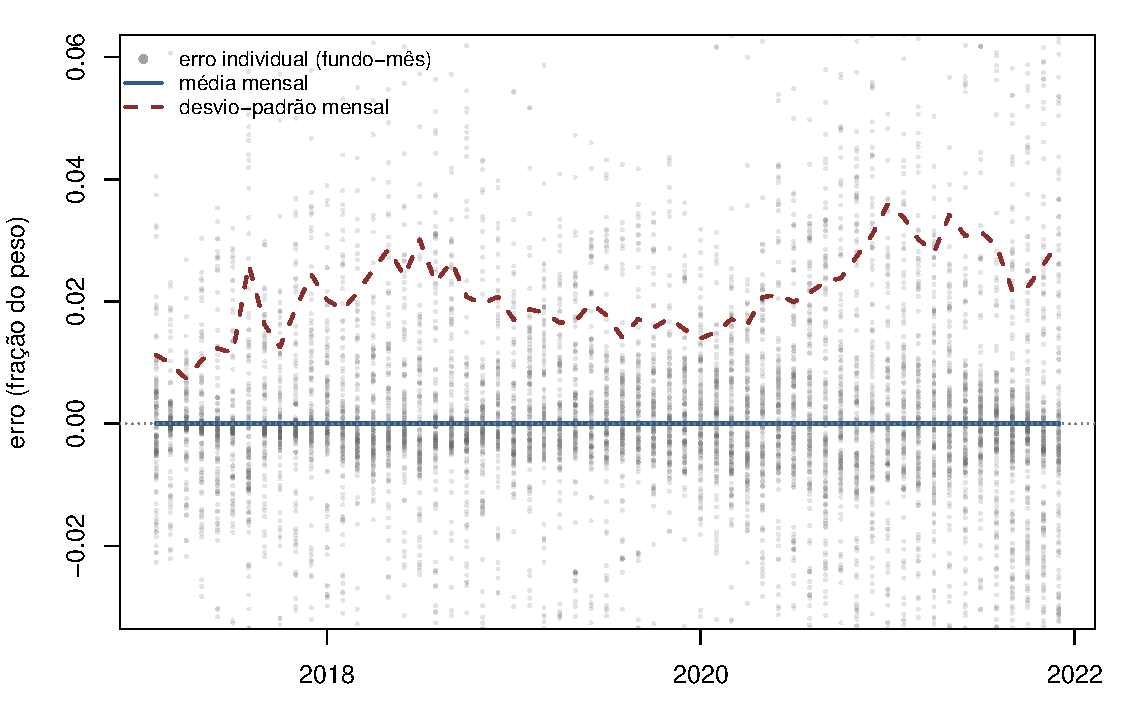
\includegraphics[width=0.75\textwidth]{fig_erro_e_mensal_v2.pdf}
\caption{Evolução mês a mês do erro $e$: nuvem cinza = erro individual de cada fundo-mês; linha
azul = média mensal (mecanicamente zero); linha vermelha tracejada = desvio-padrão mensal. Base:
VALE3--Itaú (250 fundos, 1 ativo).}
\end{figure}

\FloatBarrier
\subsection{Etapa 2: ajuste parcial}

Relembrando a equação~\eqref{eq:pa}, $w_{i,n,t+1} - w_{i,n,t} = \lambda\, d_{i,n,t} +
u_{i,n,t+1}$, com $d_{i,n,t} \equiv w^*_{i,n,t} - w_{i,n,t}$: o alvo $w^*_{i,n,t} =
g(x'_{i,n,t}\theta_{n,t})$ vem da Etapa 1 (Seção~\ref{sec:resultados}.1), e $d_{i,n,t}$ é a
distância entre a posição atual do fundo e esse alvo. O ajuste parcial modela a mudança de
posição de um mês para o outro como uma fração $\lambda$ dessa distância, estimada por MQO
pooled (Seção~\ref{sec:metodologia}) --- um único coeficiente para todo fundo e todo ativo. O
erro $u_{i,n,t+1}$ mede o quanto a mudança de posição observada difere do que essa velocidade
média de ajuste previu: valores próximos de zero indicam fundos cuja movimentação segue de perto
o $\lambda$ estimado; valores grandes indicam movimentos abruptos --- apostas concentradas de
curto prazo --- que o modelo, por construção, não tem como antecipar.

\begin{table}[h]\centering\small
\caption{Estatísticas do erro $u$, Etapa 2 (7.987 observações, pares de meses consecutivos).
Base: VALE3--Itaú (250 fundos, 1 ativo).}
\begin{tabular}{@{}lr@{}}
\toprule
Estatística & Valor \\
\midrule
Média & $0{,}0002$ \\
Desvio-padrão & $0{,}0151$ \\
Mediana & $-0{,}0004$ \\
Mínimo / Máximo & $-0{,}160$ / $0{,}185$ \\
\% de observações com $u>0$ & $44{,}3\%$ \\
Assimetria & $0{,}59$ \\
Curtose & $19{,}4$ (normal $=3$) \\
\bottomrule
\end{tabular}
\end{table}

\begin{figure}[h]\centering
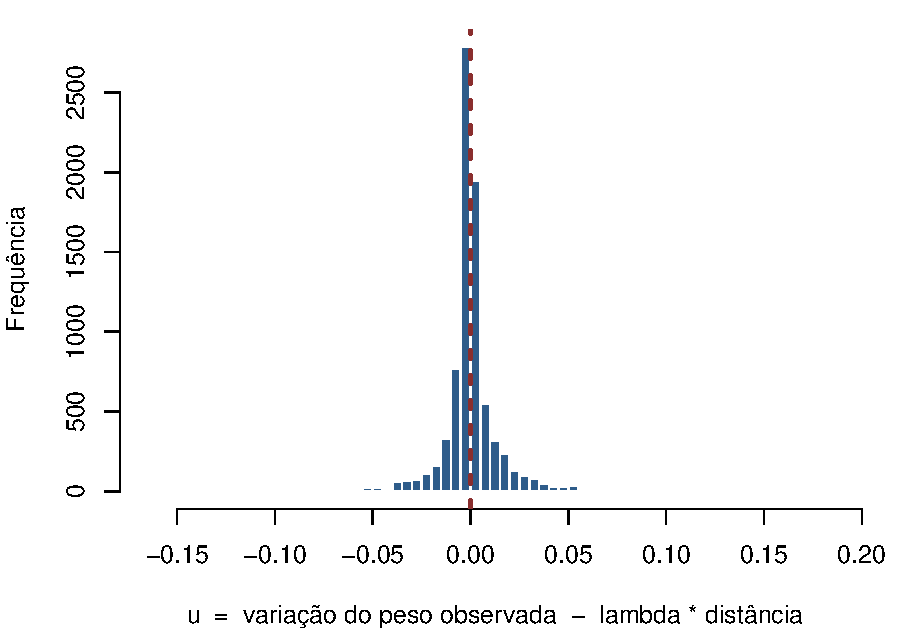
\includegraphics[width=0.65\textwidth]{hist_erro_u_v2.pdf}
\caption{Histograma do erro $u$ (7.987 observações). Base: VALE3--Itaú (250 fundos, 1 ativo).}
\end{figure}

\begin{figure}[h]\centering
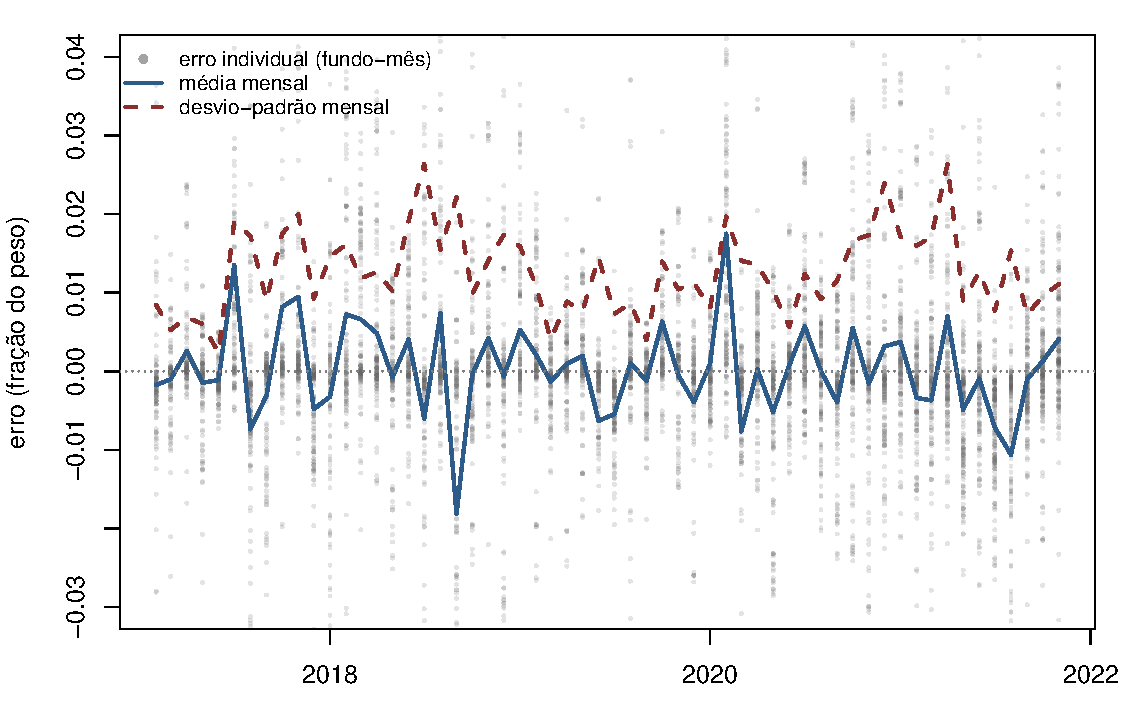
\includegraphics[width=0.75\textwidth]{fig_erro_u_mensal_v2.pdf}
\caption{Evolução mês a mês do erro $u$. Base: VALE3--Itaú (250 fundos, 1 ativo).}
\end{figure}

\FloatBarrier
\subsection{Etapa 3: esquema fora da amostra}

Relembrando a equação~\eqref{eq:oos}: $\widehat w_{i,n,t+h} = w_{i,n,t} +
\widehat\lambda_{h,\text{treino}}\, d_{i,n,t}$ (ajuste parcial) contra $\widehat w_{i,n,t+h} =
w_{i,n,t}$ (previsão ingênua), com $\lambda_h$ estimado \textbf{apenas} nos meses de treino
(anteriores a janeiro de 2020) e aplicado, fixo, aos meses de teste --- dados que o modelo nunca
viu durante a estimação (a robustez dessa escolha de $\lambda$ fixo está discutida na
Seção~\ref{sec:metodologia}). O erro fora da amostra, $\text{erro}_{i,n,t+h} =
(w_{i,n,t+h}-w_{i,n,t}) - \widehat\lambda_{h,\text{treino}}\, d_{i,n,t}$, mede o quanto essa
previsão --- feita com um parâmetro estimado em dados que o modelo nunca viu no período de teste
--- erra ao prever a mudança de posição real. É esse erro que responde à pergunta central deste
trabalho (Seção~\ref{sec:metodologia}): o ajuste parcial estimado com dados antigos ainda ajuda
a prever dados novos, ou uma previsão ingênua seria tão boa quanto? As tabelas e figuras a seguir
cobrem primeiro o caso de base ($h=1$, VALE3--Itaú), e depois a generalização completa --- todas
as gestoras, todos os ativos, quatro horizontes de previsão --- que estrutura o restante desta
subseção.

\begin{table}[h]\centering\small
\caption{RMSE e MAE dentro e fora da amostra, ajuste parcial vs. ingênua. Base: VALE3--Itaú
(250 fundos, 1 ativo).}
\begin{tabular}{@{}lrrr@{}}
\toprule
Amostra & Modelo & RMSE & MAE \\
\midrule
Treino (2017--2019) & Ajuste parcial & $0{,}01463$ & --- \\
Treino (2017--2019) & Ingênua        & $0{,}01510$ & --- \\
Teste (2020--2021)  & Ajuste parcial & $0{,}01560$ & $0{,}00906$ \\
Teste (2020--2021)  & Ingênua        & $0{,}01585$ & $0{,}00847$ \\
\bottomrule
\end{tabular}
\end{table}

\begin{figure}[h]\centering
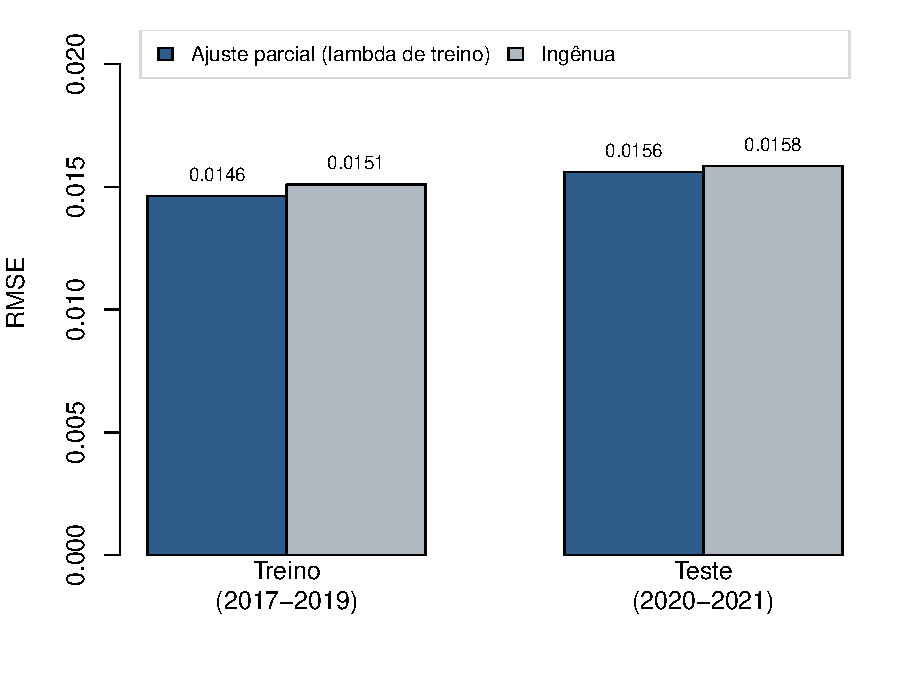
\includegraphics[width=0.6\textwidth]{fig_oos_barras_v2.pdf}
\caption{RMSE dentro (treino) e fora (teste) da amostra, ajuste parcial vs. ingênua. Base:
VALE3--Itaú (250 fundos, 1 ativo).}
\end{figure}

\begin{figure}[h]\centering
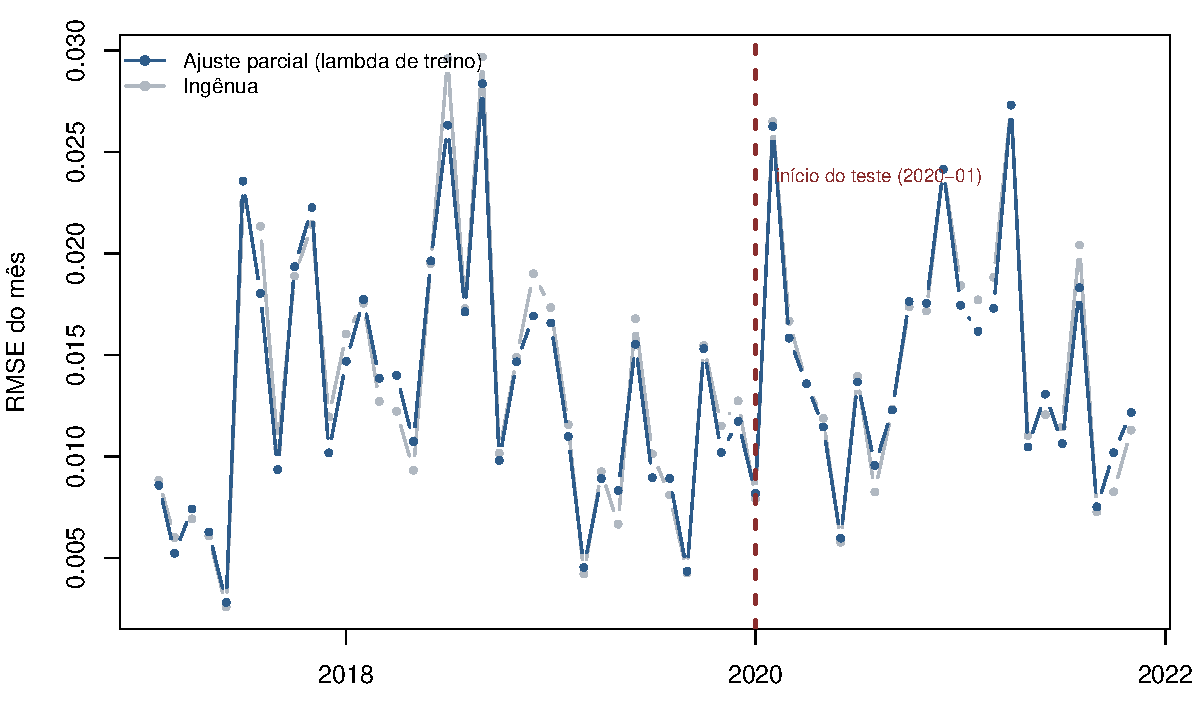
\includegraphics[width=0.78\textwidth]{fig_erro_periodo_completo_v2.pdf}
\caption{RMSE mês a mês no período completo (2017--2021). A linha vermelha tracejada marca o
início do teste (2020-01). Base: VALE3--Itaú (250 fundos, 1 ativo).}
\end{figure}

\FloatBarrier

A generalização da Etapa 3 --- índice de ativo $n$ e horizonte $h$ explícitos na
equação~\eqref{eq:pa}, conforme a Seção~\ref{sec:metodologia} --- permite ir além do RMSE
agregado acima e perguntar \emph{quem} erra mais: quais fundos, gestoras e ativos têm erro fora
da amostra pequeno e estável, e quais fogem sistematicamente do modelo. \textbf{A partir daqui, e
até o final desta subseção, todas as tabelas e figuras usam a base multiativo} (2.347 fundos,
41 gestoras, 501 ativos, Tabela~\ref{tab:amostra}) --- não mais a amostra VALE3--Itaú das seções
anteriores.

\begin{figure}[H]\centering
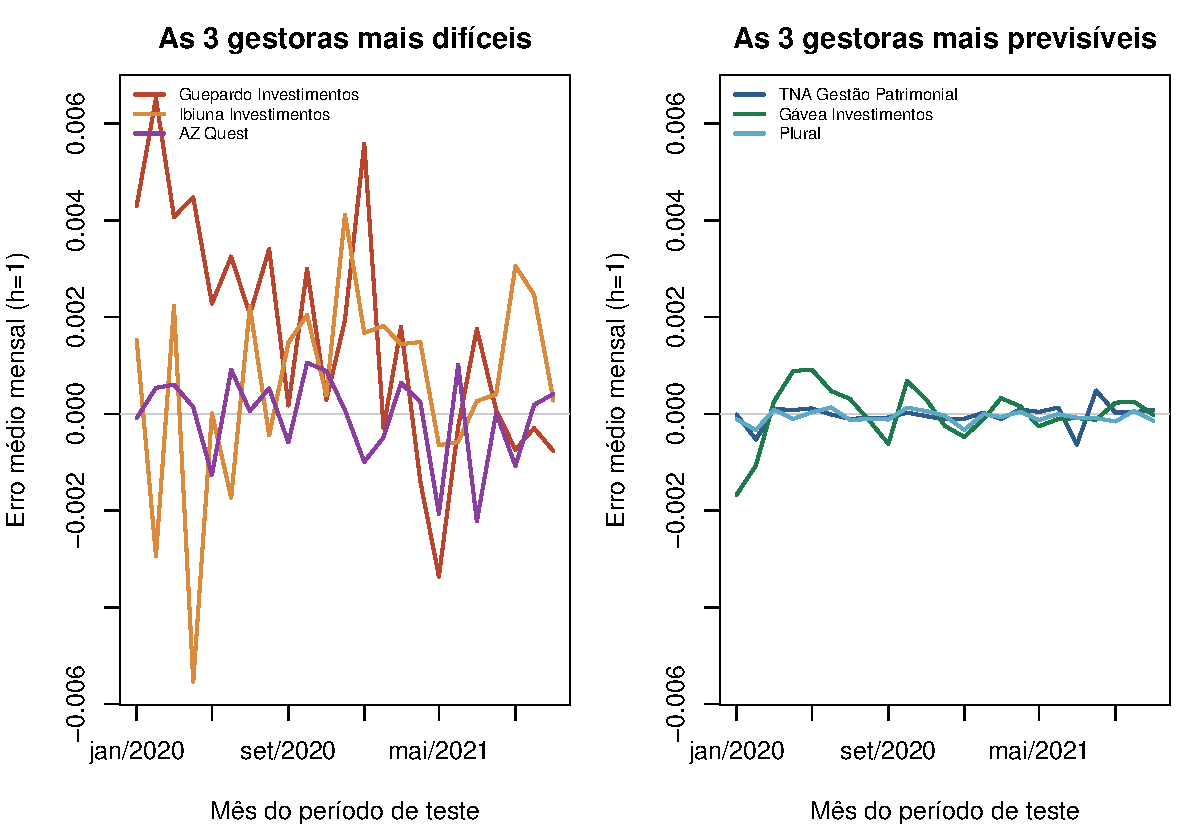
\includegraphics[width=0.95\textwidth]{fig_dinamica_erro_gestora_extremos.pdf}
\caption{Evolução mensal do erro médio fora da amostra ($h=1$), para as 3 gestoras mais
difíceis de prever e as 3 mais previsíveis em todos os horizontes testados
(Tabelas~\ref{tab:rmse-gestora} e~\ref{tab:margem-gestora}). Base: multiativo (2.347 fundos,
41 gestoras, 501 ativos).}
\label{fig:dinamica-gestora}
\end{figure}

\begin{figure}[H]\centering
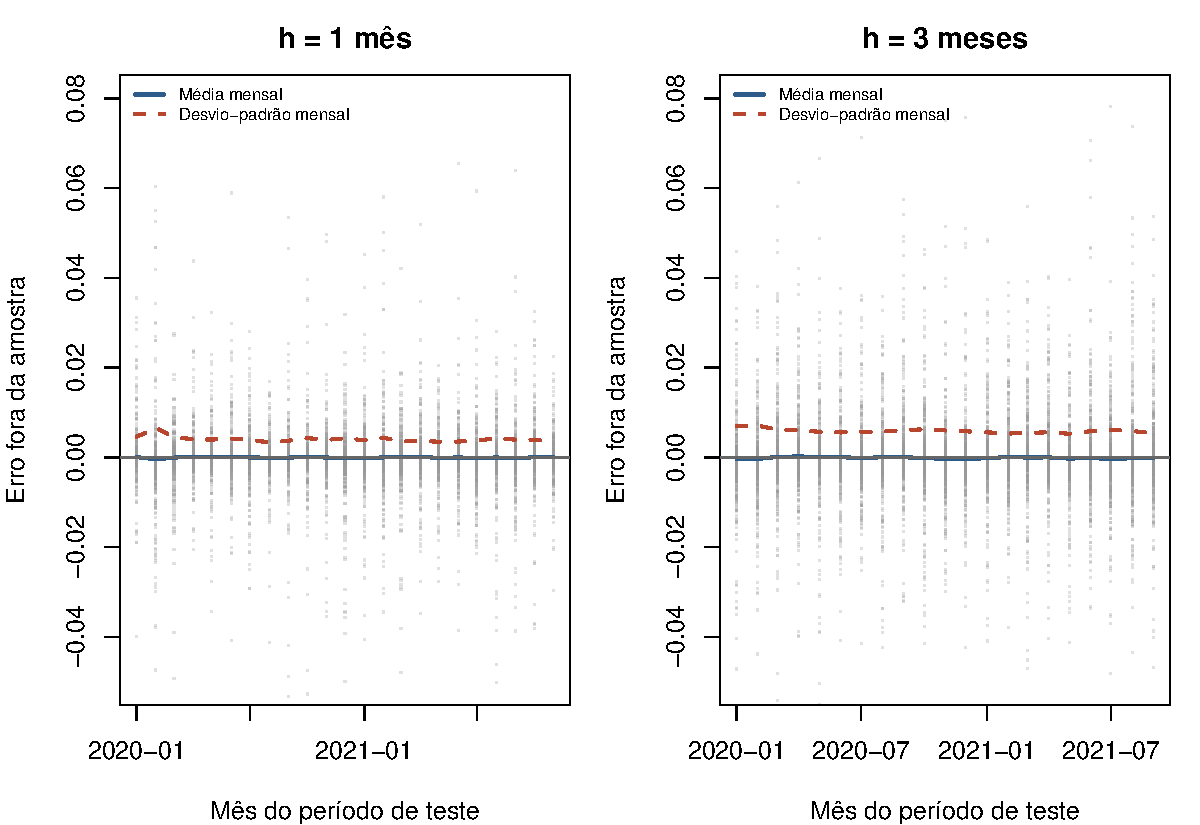
\includegraphics[width=0.95\textwidth]{fig_dinamica_erro_oos_agregado.pdf}
\caption{Erro fora da amostra ao longo do período de teste (2020--2021), agregado em todos os
fundos, gestoras e ativos --- nuvem cinza: erro individual de cada fundo-ativo-mês; linha azul:
média mensal; linha vermelha: desvio-padrão mensal. Painel esquerdo: $h=1$ mês; painel direito:
$h=3$ meses. Base: multiativo (2.347 fundos, 41 gestoras, 501 ativos).}
\label{fig:dinamica-agregado}
\end{figure}

\begin{figure}[H]\centering
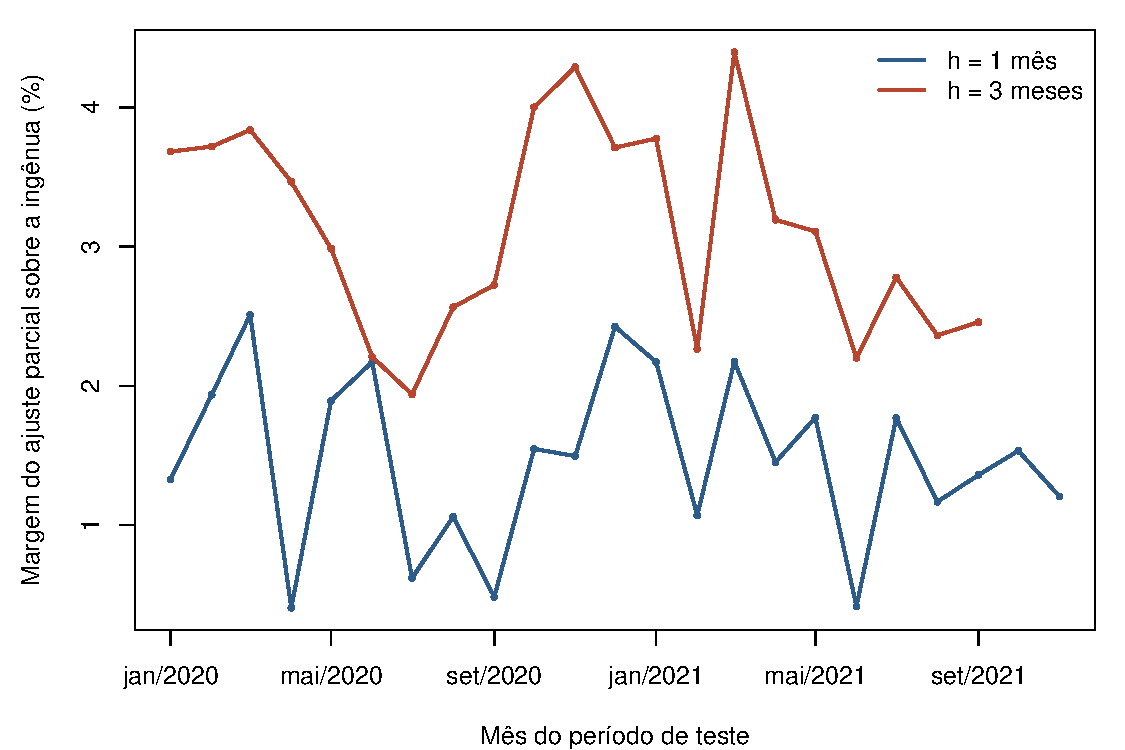
\includegraphics[width=0.75\textwidth]{fig_margem_dinamica_mensal.pdf}
\caption{Margem do ajuste parcial sobre a previsão ingênua, mês a mês, ao longo de todo o
período de teste (2020--2021) --- $h=1$ e $h=3$. Complementa a Tabela~\ref{tab:margem-gestora}
(que resume a margem do período inteiro num único número por gestora e horizonte) mostrando se
essa vantagem é estável ao longo do tempo. Base: multiativo (2.347 fundos, 41 gestoras,
501 ativos).}
\label{fig:margem-dinamica}
\end{figure}

\begin{figure}[H]\centering
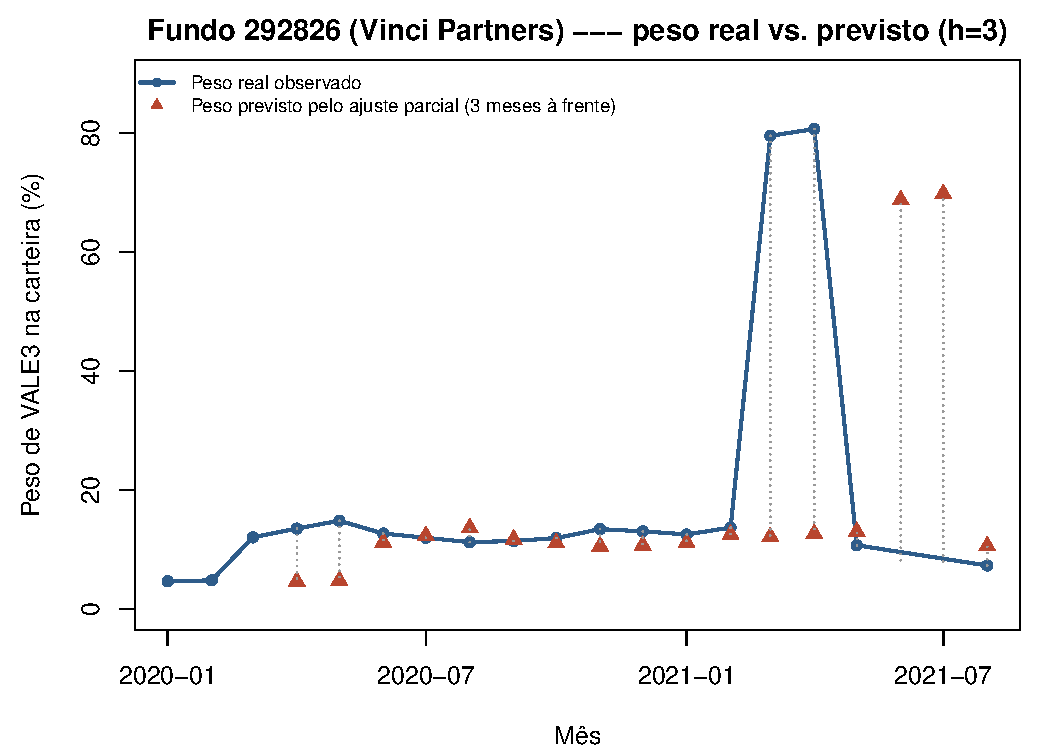
\includegraphics[width=0.78\textwidth]{fig_trajetoria_fundo_vinci_vale3.pdf}
\caption{Peso real vs. peso previsto pelo ajuste parcial ($h=3$), fundo 292826 (Vinci Partners),
em VALE3 --- o fundo com maior RMSE fora da amostra identificado neste trabalho. O modelo não
antecipa o salto de $13\%$ para $80\%$ em fev--mar/2021 (triângulos ficam perto de $12\%$
enquanto o peso real dispara), e também erra na volta: baseado nos pesos elevados recém-observados,
prevê continuidade em torno de $70\%$ quando o peso real já havia recuado para
$10$--$13\%$. Base: multiativo (2.347 fundos, 41 gestoras, 501 ativos) --- este gráfico exibe
apenas um fundo e um ativo (VALE3) dessa base, para ilustração.}
\label{fig:trajetoria-fundo}
\end{figure}

\begin{figure}[H]\centering
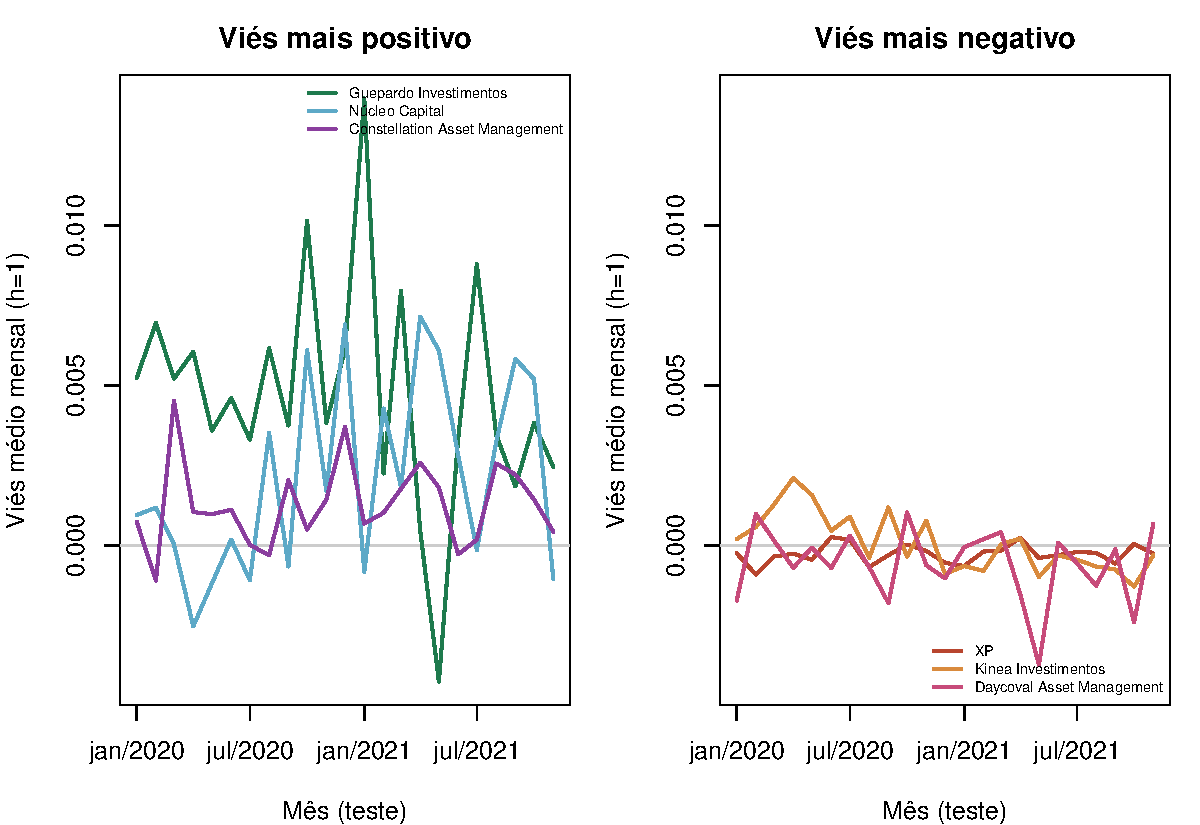
\includegraphics[width=0.95\textwidth]{fig_vies_dinamico_gestora.pdf}
\caption{Viés médio mensal fora da amostra ($h=1$, com sinal --- não apenas magnitude), para as
3 gestoras com viés mais positivo e as 3 com viés mais negativo (entre gestoras com pelo menos
100 observações de teste). Pergunta diferente da magnitude do erro: quem compra ou vende
sistematicamente mais do que o modelo prevê. Base: multiativo (2.347 fundos, 41 gestoras,
501 ativos).}
\label{fig:vies-dinamico}
\end{figure}

\paragraph{O viés é persistente, mas explica pouco do erro.} Um viés grande e estável seria
evidência de que uma gestora tem um estilo sistemático (convicção própria, mandato diferente)
não capturado pelas cinco características do modelo --- vale então perguntar se o padrão da
Figura~\ref{fig:vies-dinamico} é um traço real da gestora ou um acidente da janela de teste.
Dividindo os 23 meses de teste ao meio e comparando o viés médio de cada gestora nas duas
metades, a correlação é $0{,}83$ ($R^2=0{,}69$, $p<0{,}0001$): o viés é, de fato, persistente.

\begin{figure}[H]\centering
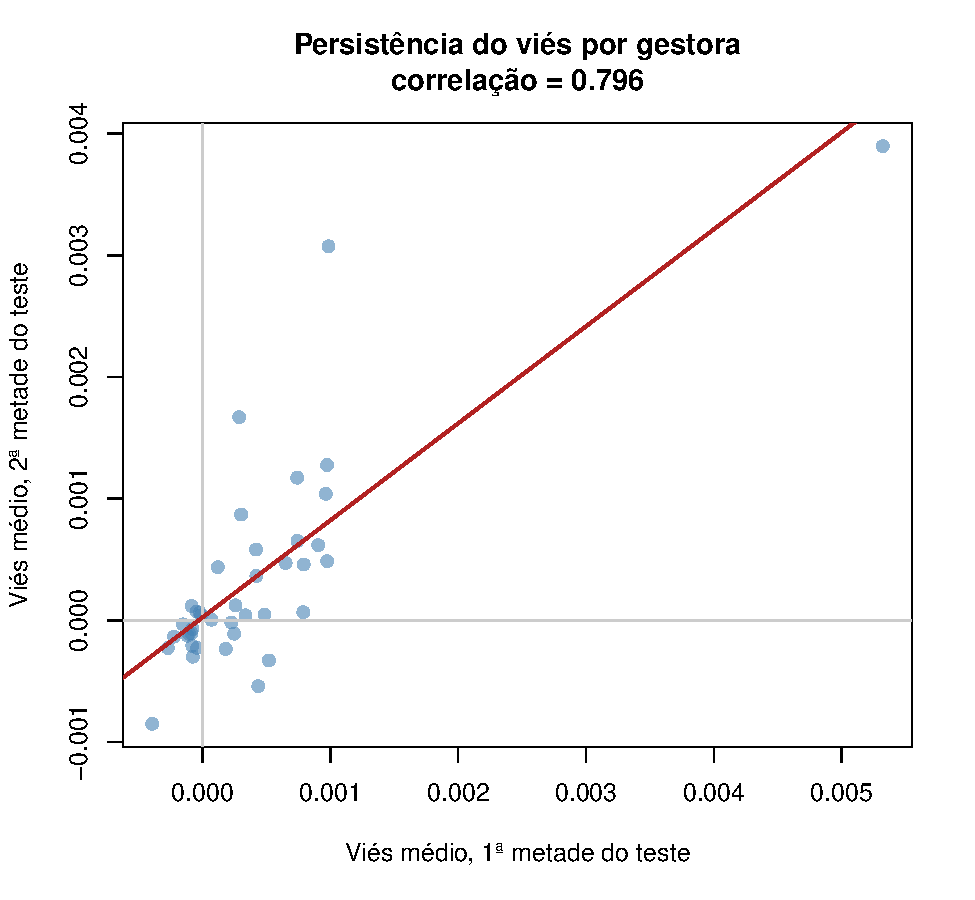
\includegraphics[width=0.55\textwidth]{fig_persistencia_vies_gestora.pdf}
\caption{Persistência do viés por gestora: viés médio na 1ª metade do período de teste
(2020-01 a 2020-12) vs.\ na 2ª metade (2021-01 a 2021-11), 40 gestoras com pelo menos 50
observações em cada metade. Base: multiativo (2.347 fundos, 41 gestoras, 501 ativos).}
\label{fig:persistencia-vies}
\end{figure}

Sendo persistente, o viés poderia em princípio ser corrigido: estimando-o só na 1ª metade do
teste e aplicando-o, como um ajuste fixo, às previsões da 2ª metade (que nunca entraram nessa
estimativa), o RMSE agregado da 2ª metade cai de $0{,}006093$ para $0{,}006089$ --- uma melhora
de apenas $0{,}07\%$. A correção ajuda mais nas gestoras com viés mais extremo (Guepardo
Investimentos, $-3{,}7\%$ de RMSE; Real Investor, $-3{,}3\%$; Núcleo Capital, $-3{,}2\%$), mas é
irrelevante para a maioria. A razão fica clara na decomposição a seguir.

\paragraph{Por que o viés importa pouco: a variância domina o erro.} Como
$\text{RMSE}^2 = \text{viés}^2 + \text{variância}$, é possível medir exatamente que fração do
erro de cada gestora vem do viés (um deslocamento sistemático, corrigível) e que fração vem da
variância (dispersão em torno da média, não corrigível por um simples ajuste de nível).

\begin{figure}[H]\centering
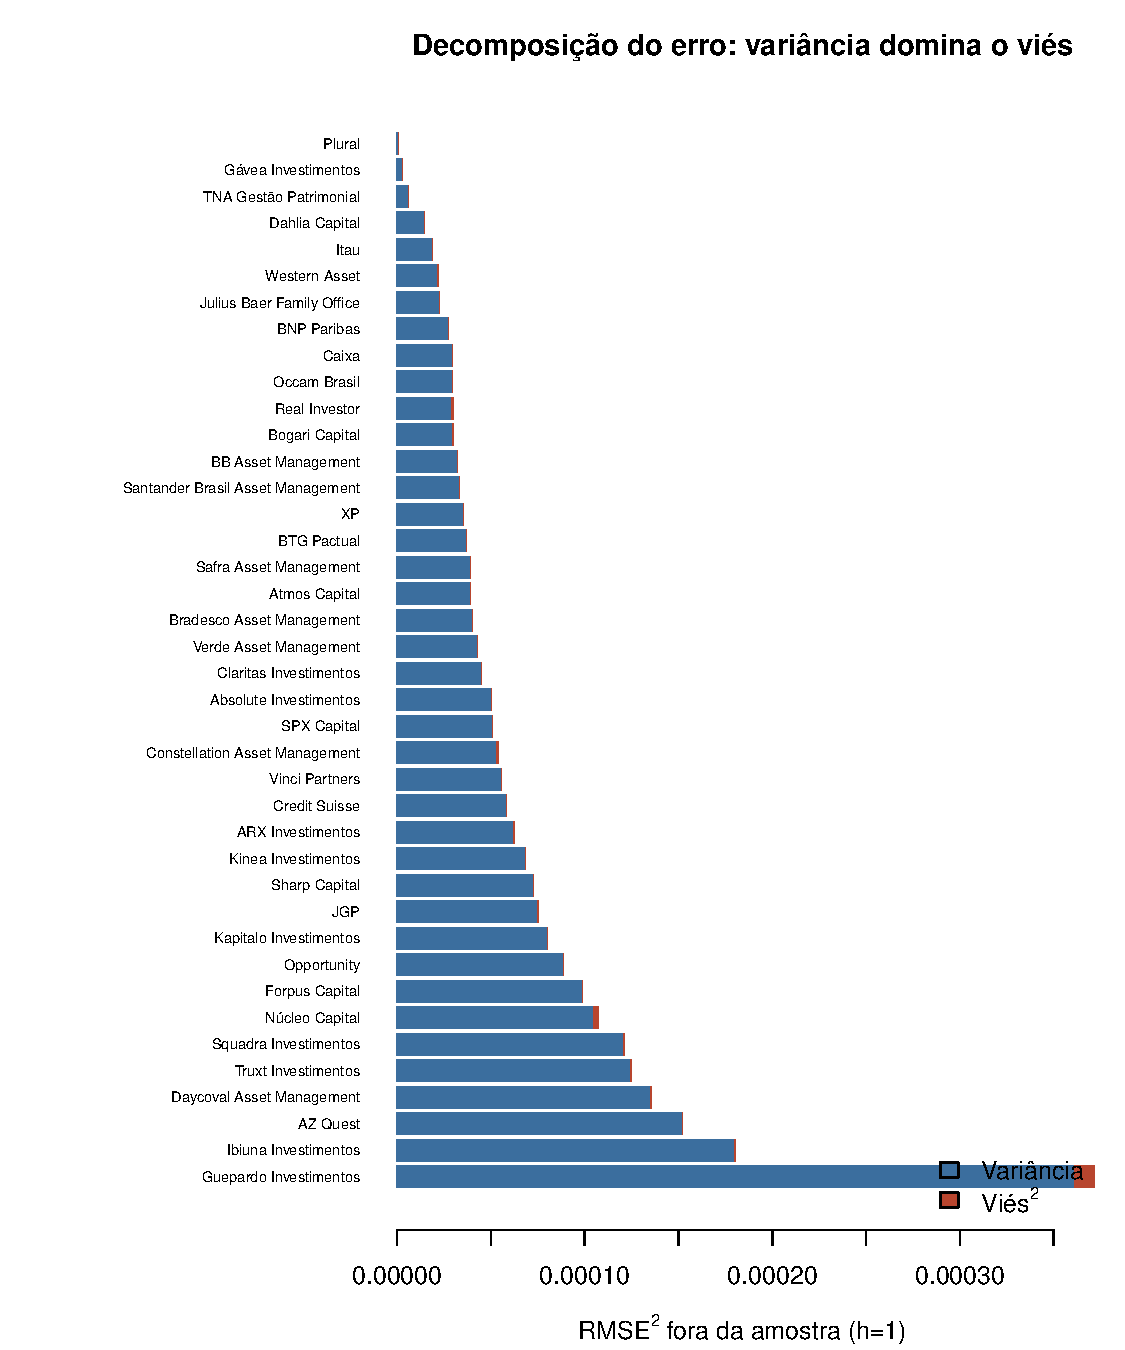
\includegraphics[width=0.68\textwidth]{fig_decomposicao_vies_variancia.pdf}
\caption{Decomposição $\text{RMSE}^2=\text{viés}^2+\text{variância}$ do erro fora da amostra
($h=1$), por gestora, ordenada por RMSE. Base: multiativo (2.347 fundos, 41 gestoras,
501 ativos).}
\label{fig:decomposicao-vies-variancia}
\end{figure}

Em média entre as 40 gestoras, o viés$^2$ explica só $0{,}67\%$ do $\text{RMSE}^2$ (mediana
$0{,}16\%$); mesmo a Guepardo, a mais enviesada, chega a apenas $5{,}96\%$. Somando todas as
observações da base (\emph{pooled}, em vez de médias por gestora), o viés$^2$ é essencialmente
$0\%$ do erro total. A variância --- não o viés --- é, de longe, a peça que domina o erro fora
da amostra, o que explica por que a correção acima rende tão pouco.

\paragraph{A variância também é persistente.} Se a variância domina o erro, vale perguntar se
ela também é um traço estável da gestora ou apenas ruído ano a ano. Repetindo o teste de
persistência (1ª vs.\ 2ª metade do teste), agora para o desvio-padrão do erro em vez da média:
correlação de $0{,}78$ ($R^2=0{,}61$, $p<0{,}0001$) --- quase tão persistente quanto o viés.
Gestoras mais imprevisíveis continuam mais imprevisíveis de um período para o outro.

\begin{figure}[H]\centering
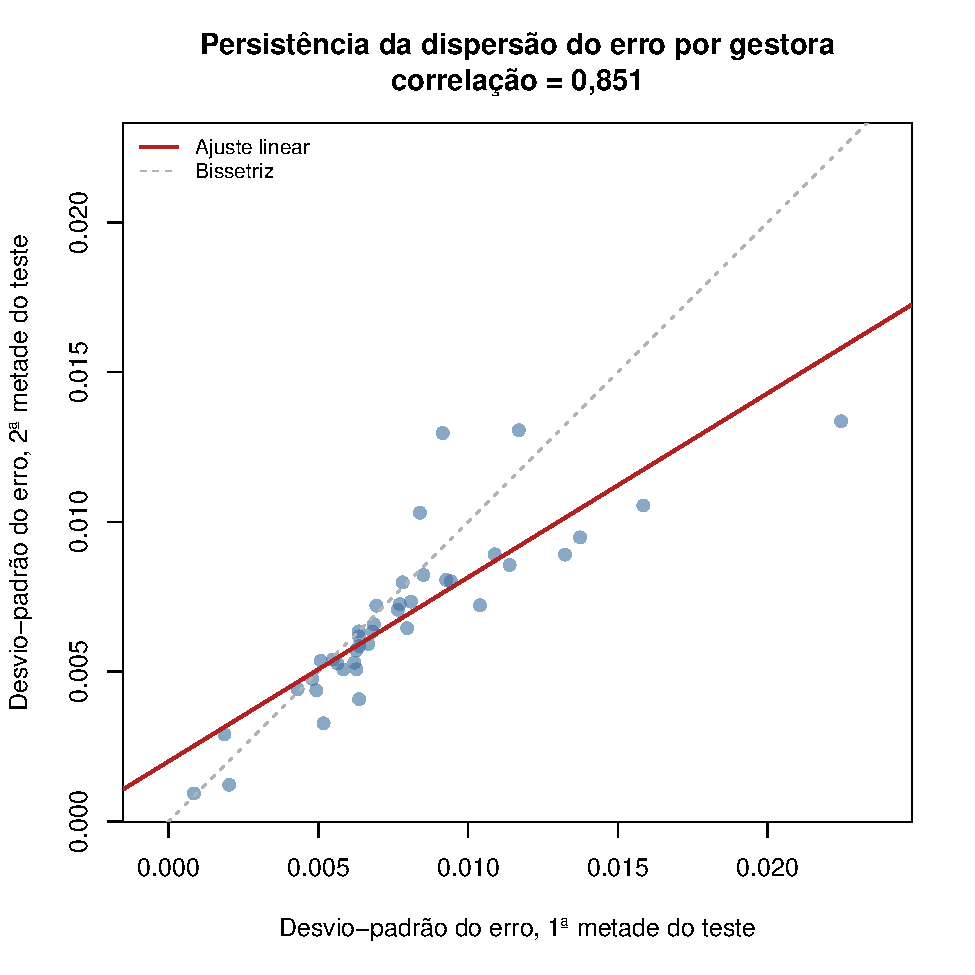
\includegraphics[width=0.55\textwidth]{fig_persistencia_dp_gestora.pdf}
\caption{Persistência da dispersão do erro por gestora: desvio-padrão do erro na 1ª metade do
teste vs.\ na 2ª metade, mesmas 40 gestoras da Figura~\ref{fig:persistencia-vies}. A linha
tracejada é a identidade ($y=x$); a linha sólida é o ajuste linear. Base: multiativo
(2.347 fundos, 41 gestoras, 501 ativos).}
\label{fig:persistencia-dp}
\end{figure}

\paragraph{O que explica a variância: concentração da carteira, mais do que beta ou tamanho.}
Sendo a variância a peça relevante do erro, e sendo ela previsível de uma gestora para a outra,
cabe perguntar o que a determina. Cruzando o desvio-padrão do erro de cada gestora contra três
características --- beta médio do fundo, tamanho médio (log do PL) e concentração média da
carteira (índice HHI dos pesos por ativo, dentro de cada fundo-mês) --- a concentração se destaca
claramente: correlação de $0{,}76$ ($R^2=0{,}57$), contra $0{,}49$ ($R^2=0{,}24$) do beta e
apenas $0{,}14$ ($R^2=0{,}02$) do tamanho.

\begin{figure}[H]\centering
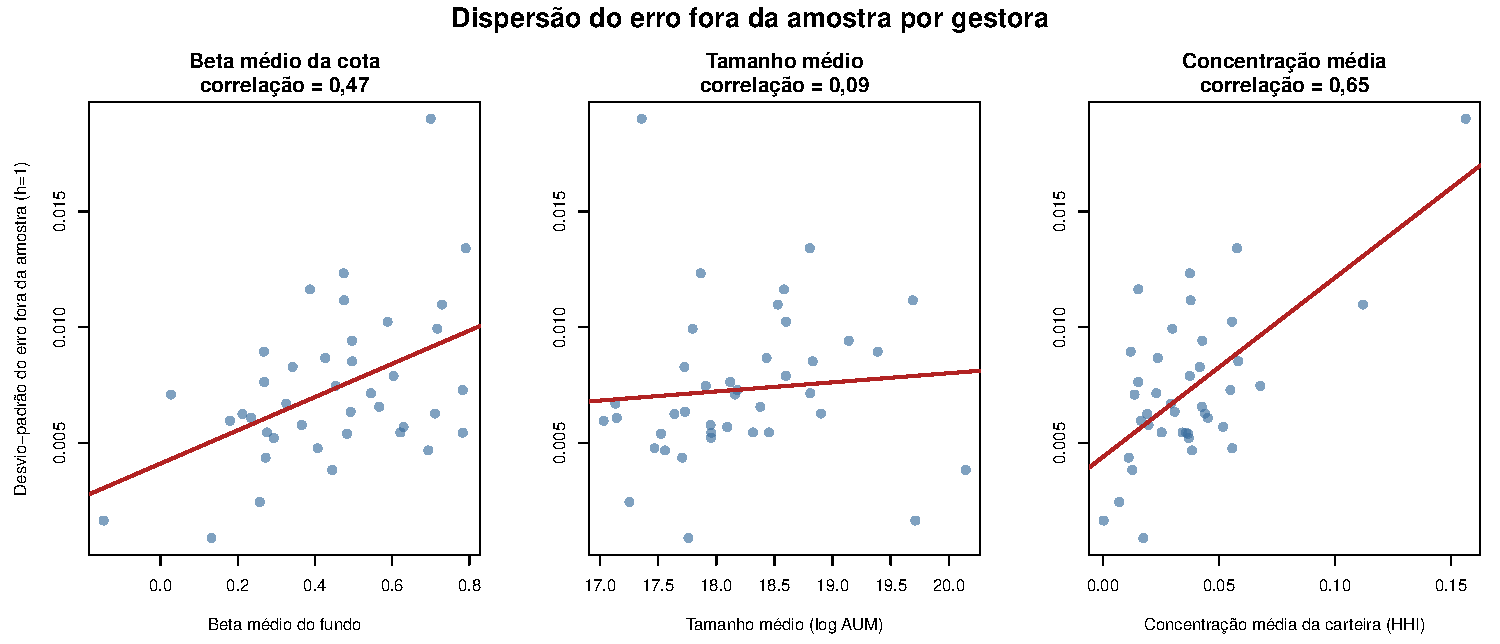
\includegraphics[width=0.95\textwidth]{fig_explica_variancia_gestora.pdf}
\caption{Desvio-padrão do erro fora da amostra por gestora ($h=1$) vs.\ beta médio do fundo,
tamanho médio (log AUM) e concentração média da carteira (HHI), 40 gestoras. Base: multiativo
(2.347 fundos, 41 gestoras, 501 ativos).}
\label{fig:explica-variancia}
\end{figure}

Numa regressão múltipla com as três características juntas, só a concentração continua
estatisticamente significativa ($t=5{,}48$, $p<0{,}0001$); beta e tamanho perdem significância.
Isso sugere que a relação entre beta e RMSE mostrada na Figura~\ref{fig:beta-erro} a seguir é, em
boa parte, um reflexo indireto da concentração --- gestoras com fundos de beta alto tendem
também a manter carteiras mais concentradas, e é a concentração, não o beta em si, que parece
determinar o quão imprevisível é a mudança de posição.

\paragraph{Concentração no nível fundo-mês: sobretudo um traço entre fundos, não dentro do
fundo.} O resultado acima usa uma única média de concentração por gestora --- 40 pontos. Refinado
para o nível fundo-mês --- a concentração da carteira de um fundo específico, num mês específico,
contra o erro desse mesmo fundo nesse mesmo mês, com dezenas de milhares de pares em vez de 40 ---
o padrão se confirma e se aprofunda em três versões.

\begin{figure}[H]\centering
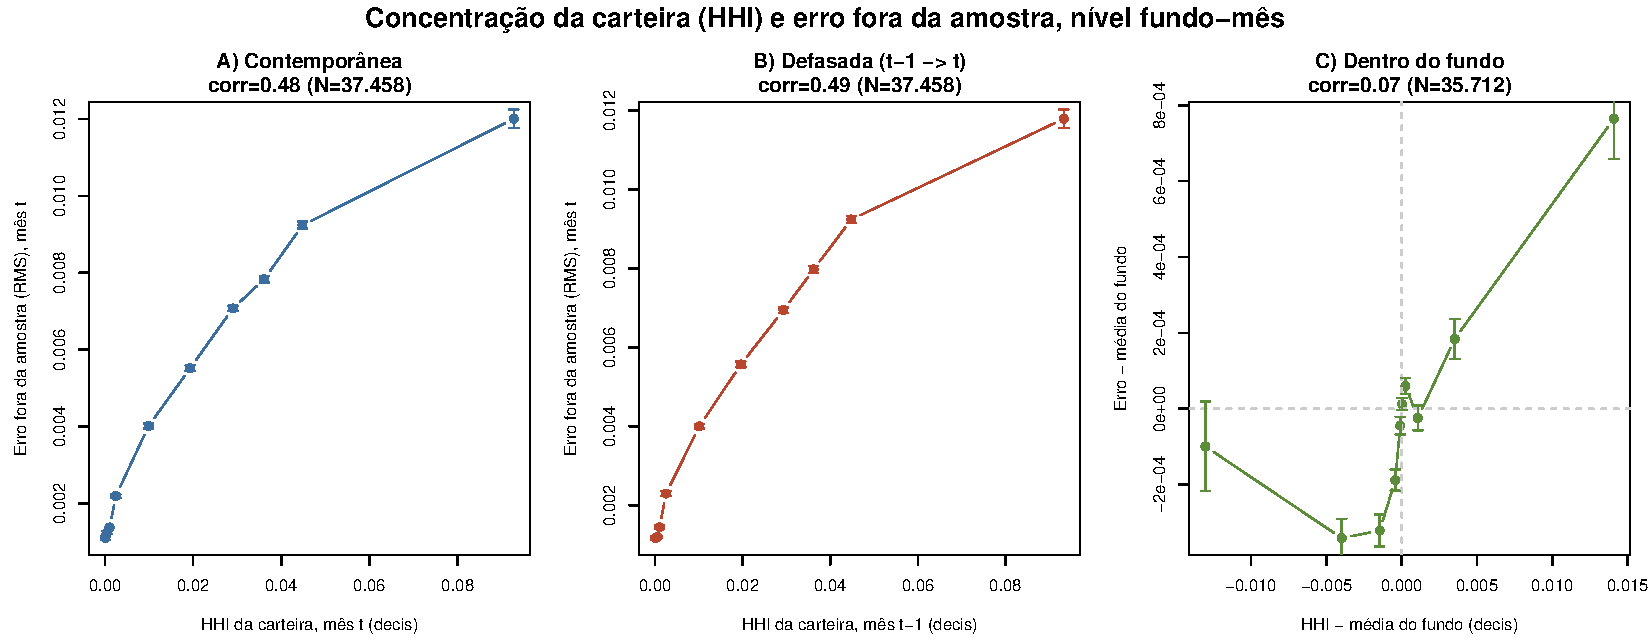
\includegraphics[width=0.95\textwidth]{fig_concentracao_mes_a_mes.pdf}
\caption{Concentração da carteira (HHI) vs.\ erro fora da amostra (RMS), nível fundo-mês, em
decis. (A) contemporânea: HHI do mês $t$ vs.\ erro do mês $t$. (B) defasada: HHI do mês $t-1$
vs.\ erro do mês $t$. (C) dentro do fundo: ambos os eixos com a média de cada fundo subtraída,
isolando a variação temporal dentro do mesmo fundo. Barras de erro $=\pm 1$ erro-padrão da média
por decil. Base: multiativo (2.347 fundos, 41 gestoras, 501 ativos).}
\label{fig:concentracao-mes}
\end{figure}

Nas versões contemporânea e defasada (painéis A e B), a correlação é praticamente idêntica
($0{,}42$ e $0{,}44$) --- a concentração do mês \emph{anterior}, que já era conhecida antes do
erro acontecer, prediz o erro do mês seguinte quase tão bem quanto a concentração do próprio mês,
afastando a hipótese de que a relação seja só uma coincidência dentro do mesmo mês. Já a versão
dentro do fundo (painel C, que subtrai de cada fundo sua própria média de concentração e de erro,
isolando a variação temporal de um mesmo fundo em relação a si mesmo) mostra uma correlação bem
mais fraca ($0{,}21$): a concentração é, sobretudo, um traço que diferencia fundos \emph{entre
si} --- um fundo tipicamente mais concentrado do que a média tende a errar mais do que a média
--- e não tanto um sinal de curto prazo de que um fundo específico está prestes a errar mais do
que o normal dele mesmo.

\begin{figure}[H]\centering
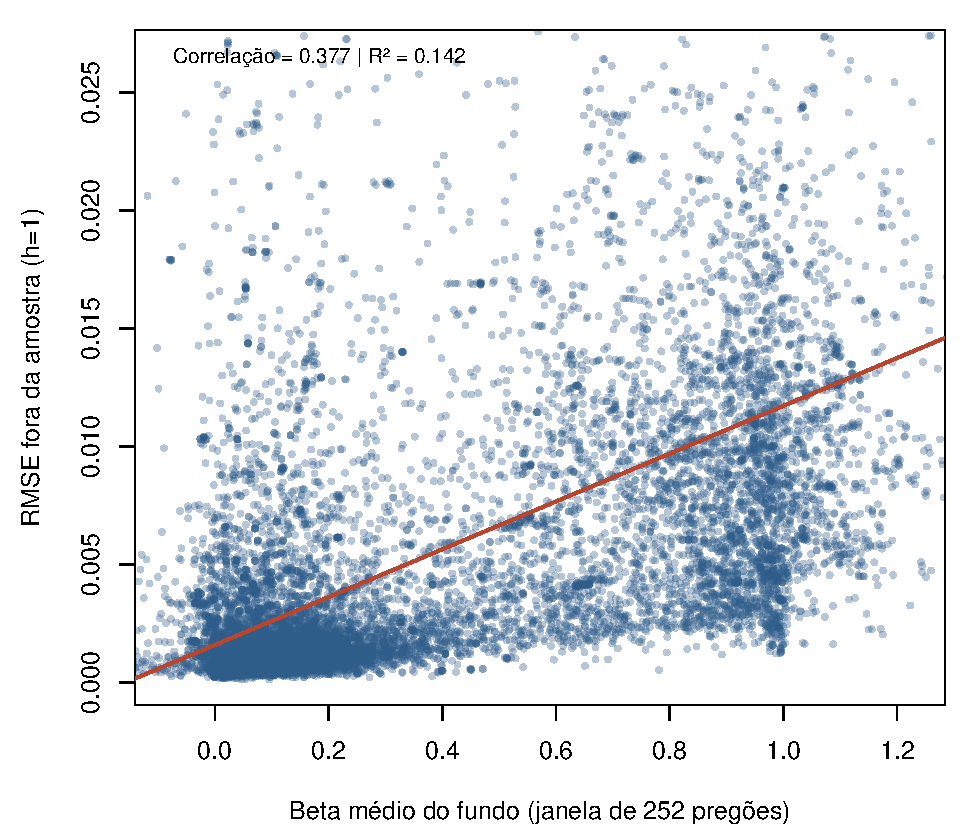
\includegraphics[width=0.68\textwidth]{fig_beta_vs_erro.pdf}
\caption{Beta médio do fundo (Etapa 1) vs. RMSE fora da amostra ($h=1$), 1.946 fundos com pelo
menos 6 observações de teste, após o mesmo filtro de posição-poeira usado nas demais figuras
(peso mediano da célula fundo-ativo $\geq 0{,}1\%$). A característica que mais explica o
\emph{peso} (Tabela~\ref{tab:theta}) também explica parte de quem é mais difícil de prever
\emph{fora da amostra}: $R^2=0{,}23$. Base: multiativo (2.347 fundos, 41 gestoras, 501 ativos)
--- o beta do fundo usado aqui é o mesmo conceito estimado na Etapa 1, recalculado nessa base
maior.}
\label{fig:beta-erro}
\end{figure}

\begin{figure}[H]\centering
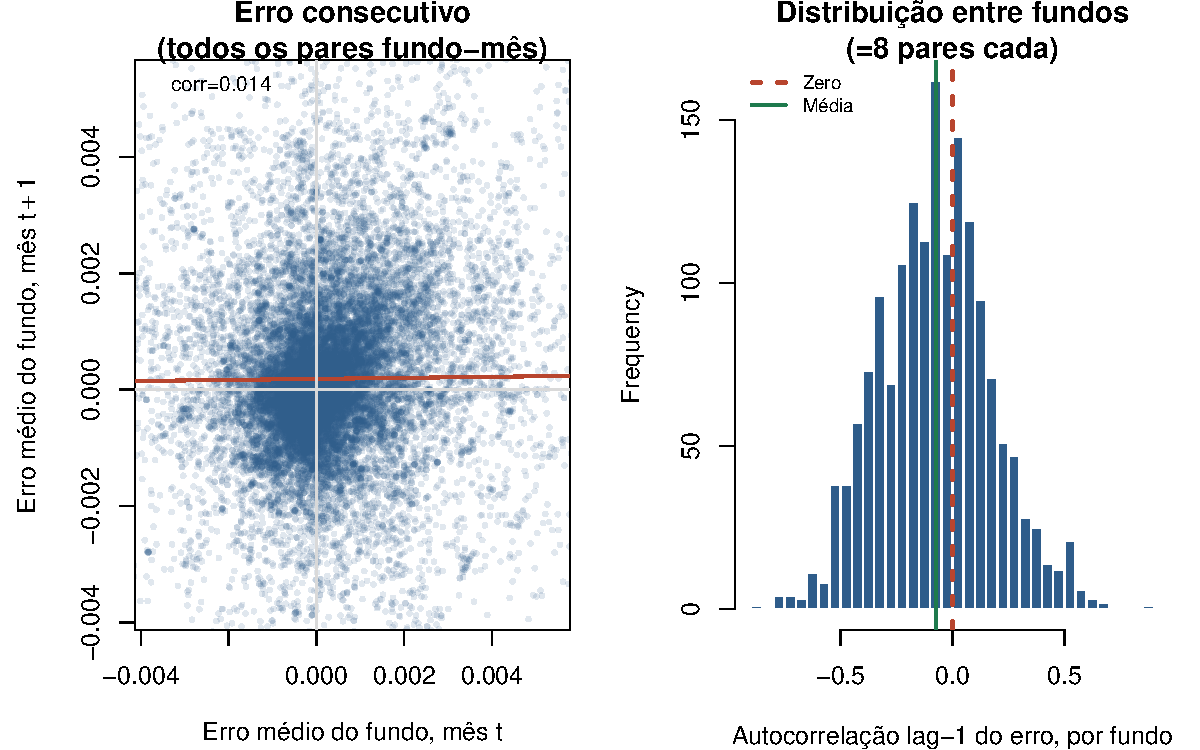
\includegraphics[width=0.95\textwidth]{fig_persistencia_erro.pdf}
\caption{Persistência do erro fora da amostra dentro do mesmo fundo: erro médio no mês $t$ vs.
erro médio no mês $t+1$ (agregado por fundo-mês, 34.120 pares consecutivos, 1.923 fundos), e
distribuição da autocorrelação lag-1 entre os 1.657 fundos com pelo menos 8 pares. Correlação
pooled $=0{,}014$; autocorrelação média entre fundos $=-0{,}075$ --- sem evidência de
persistência mês a mês na \emph{direção} do erro, distinto da estabilidade de \emph{magnitude}
(RMSE) entre horizontes mostrada na Figura a seguir. Base: multiativo (2.347 fundos, 41 gestoras,
501 ativos).}
\label{fig:persistencia-erro}
\end{figure}

\begin{figure}[H]\centering
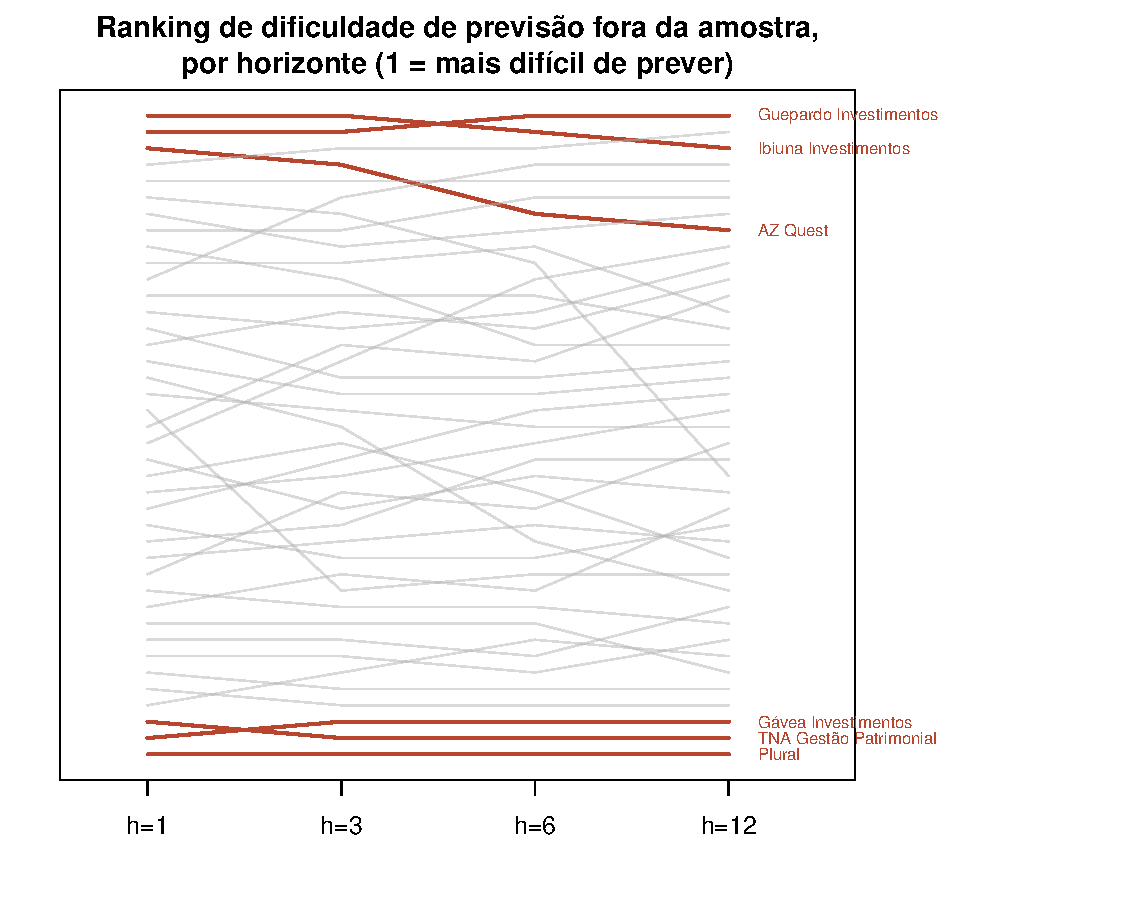
\includegraphics[width=0.75\textwidth]{fig_ranking_horizontes_slopegraph.pdf}
\caption{Estabilidade do ranking de dificuldade de previsão (RMSE fora da amostra) entre os 4
horizontes testados, 40 gestoras com dado completo em todos os horizontes (exclui Legacy
Capital, que só tem observação em $h=1$). As gestoras mais extremas (destacadas) permanecem nos
extremos em todos os horizontes; a correlação de Spearman entre rankings varia de $0{,}90$
($h=1$ vs.\ $h=12$, os mais distantes) a $0{,}99$ ($h=6$ vs.\ $h=12$, os mais próximos). Base:
multiativo (2.347 fundos, 41 gestoras, 501 ativos).}
\label{fig:ranking-horizontes}
\end{figure}

\begin{center}\scriptsize
\begin{longtable}{@{}lrrrrr@{}}
\caption{RMSE fora da amostra por gestora, todos os 430 ativos com par (treino, teste) válido
em $h=1$ --- dos 501 ativos da amostra final, 71 não têm cobertura suficiente nesse horizonte
--- em 4 horizontes, ordenado do mais ao menos errante em $h=1$. Base: multiativo (2.347 fundos,
41 gestoras, 501 ativos).}
\label{tab:rmse-gestora}\\
\toprule
Gestora & Fundos ($h{=}1$) & RMSE $h{=}1$ & RMSE $h{=}3$ & RMSE $h{=}6$ & RMSE $h{=}12$ \\
\midrule
\endfirsthead
\multicolumn{6}{l}{\textit{(continuação)}}\\
\toprule
Gestora & Fundos ($h{=}1$) & RMSE $h{=}1$ & RMSE $h{=}3$ & RMSE $h{=}6$ & RMSE $h{=}12$ \\
\midrule
\endhead
\midrule
\multicolumn{6}{r}{\textit{continua na próxima página}}\\
\endfoot
\bottomrule
\endlastfoot
Guepardo Investimentos & 10 & $0{,}01447$ & $0{,}02392$ & $0{,}03569$ & $0{,}06177$ \\
Ibiuna Investimentos & 7 & $0{,}01331$ & $0{,}02130$ & $0{,}02491$ & $0{,}02828$ \\
AZ Quest & 22 & $0{,}01096$ & $0{,}01461$ & $0{,}01649$ & $0{,}01876$ \\
Núcleo Capital & 17 & $0{,}01045$ & $0{,}01830$ & $0{,}02490$ & $0{,}03539$ \\
Squadra Investimentos & 14 & $0{,}01007$ & $0{,}01390$ & $0{,}01681$ & $0{,}02127$ \\
Forpus Capital & 3 & $0{,}00991$ & $0{,}01430$ & $0{,}01641$ & $0{,}01661$ \\
Sharp Capital & 34 & $0{,}00813$ & $0{,}01295$ & $0{,}01709$ & $0{,}02092$ \\
Truxt Investimentos & 31 & $0{,}00812$ & $0{,}01261$ & $0{,}01596$ & $0{,}01952$ \\
Legacy Capital & 1 & $0{,}00800$ & --- & --- & --- \\
ARX Investimentos & 12 & $0{,}00792$ & $0{,}01084$ & $0{,}01262$ & $0{,}01515$ \\
Vinci Partners & 48 & $0{,}00753$ & $0{,}01053$ & $0{,}01031$ & $0{,}01272$ \\
Kinea Investimentos & 4 & $0{,}00717$ & $0{,}01160$ & $0{,}01515$ & $0{,}01543$ \\
Constellation Asset Management & 26 & $0{,}00693$ & $0{,}01377$ & $0{,}01845$ & $0{,}02775$ \\
Opportunity & 19 & $0{,}00678$ & $0{,}01052$ & $0{,}01352$ & $0{,}01594$ \\
SPX Capital & 35 & $0{,}00613$ & $0{,}00916$ & $0{,}01166$ & $0{,}01328$ \\
Atmos Capital & 28 & $0{,}00613$ & $0{,}00999$ & $0{,}01340$ & $0{,}01704$ \\
Verde Asset Management & 14 & $0{,}00600$ & $0{,}01021$ & $0{,}01293$ & $0{,}01632$ \\
Absolute Investimentos & 7 & $0{,}00589$ & $0{,}00925$ & $0{,}01216$ & $0{,}01401$ \\
Daycoval Asset Management & 5 & $0{,}00582$ & $0{,}00733$ & $0{,}00741$ & $0{,}00787$ \\
JGP & 40 & $0{,}00554$ & $0{,}00773$ & $0{,}00893$ & $0{,}01074$ \\
Kapitalo Investimentos & 22 & $0{,}00538$ & $0{,}00580$ & $0{,}00690$ & $0{,}00823$ \\
Credit Suisse & 65 & $0{,}00537$ & $0{,}00750$ & $0{,}00868$ & $0{,}00980$ \\
Bogari Capital & 14 & $0{,}00533$ & $0{,}00932$ & $0{,}01209$ & $0{,}01594$ \\
Real Investor & 5 & $0{,}00486$ & $0{,}00897$ & $0{,}01412$ & $0{,}01756$ \\
Claritas Investimentos & 10 & $0{,}00481$ & $0{,}00709$ & $0{,}00795$ & $0{,}00843$ \\
Caixa & 27 & $0{,}00461$ & $0{,}00681$ & $0{,}00888$ & $0{,}01141$ \\
Bradesco Asset Management & 281 & $0{,}00443$ & $0{,}00613$ & $0{,}00728$ & $0{,}00858$ \\
Western Asset & 26 & $0{,}00437$ & $0{,}00700$ & $0{,}00960$ & $0{,}01252$ \\
BB Asset Management & 103 & $0{,}00413$ & $0{,}00642$ & $0{,}00804$ & $0{,}00989$ \\
Occam Brasil & 26 & $0{,}00411$ & $0{,}00668$ & $0{,}00763$ & $0{,}01001$ \\
BTG Pactual & 139 & $0{,}00409$ & $0{,}00611$ & $0{,}00716$ & $0{,}00880$ \\
Santander Brasil Asset Management & 70 & $0{,}00394$ & $0{,}00551$ & $0{,}00630$ & $0{,}00735$ \\
Safra Asset Management & 137 & $0{,}00360$ & $0{,}00509$ & $0{,}00603$ & $0{,}00674$ \\
Julius Baer Family Office & 57 & $0{,}00308$ & $0{,}00416$ & $0{,}00497$ & $0{,}00570$ \\
BNP Paribas & 42 & $0{,}00300$ & $0{,}00434$ & $0{,}00527$ & $0{,}00692$ \\
XP & 87 & $0{,}00294$ & $0{,}00444$ & $0{,}00537$ & $0{,}00745$ \\
Itaú & 440 & $0{,}00264$ & $0{,}00389$ & $0{,}00473$ & $0{,}00557$ \\
Dahlia Capital & 18 & $0{,}00247$ & $0{,}00426$ & $0{,}00556$ & $0{,}00625$ \\
TNA Gestão Patrimonial & 29 & $0{,}00151$ & $0{,}00218$ & $0{,}00281$ & $0{,}00388$ \\
Gávea Investimentos & 17 & $0{,}00144$ & $0{,}00265$ & $0{,}00363$ & $0{,}00470$ \\
Plural & 1 & $0{,}00050$ & $0{,}00080$ & $0{,}00105$ & $0{,}00136$ \\
\end{longtable}
\end{center}

\begin{center}\scriptsize
\begin{longtable}{@{}lrrrr@{}}
\caption{Margem do ajuste parcial sobre a ingênua ($\%$ de redução de RMSE), por gestora, 4
horizontes --- mesma ordem da Tabela~\ref{tab:rmse-gestora}. Negativo = ajuste parcial pior que
a ingênua. Base: multiativo (2.347 fundos, 41 gestoras, 501 ativos).}
\label{tab:margem-gestora}\\
\toprule
Gestora & Margem $h{=}1$ & Margem $h{=}3$ & Margem $h{=}6$ & Margem $h{=}12$ \\
\midrule
\endfirsthead
\multicolumn{5}{l}{\textit{(continuação)}}\\
\toprule
Gestora & Margem $h{=}1$ & Margem $h{=}3$ & Margem $h{=}6$ & Margem $h{=}12$ \\
\midrule
\endhead
\midrule
\multicolumn{5}{r}{\textit{continua na próxima página}}\\
\endfoot
\bottomrule
\endlastfoot
Guepardo Investimentos & $-0{,}4\%$ & $-2{,}7\%$ & $-6{,}4\%$ & $-10{,}8\%$ \\
Ibiuna Investimentos & $3{,}1\%$ & $6{,}9\%$ & $8{,}2\%$ & $14{,}9\%$ \\
AZ Quest & $3{,}2\%$ & $6{,}9\%$ & $9{,}9\%$ & $15{,}0\%$ \\
Núcleo Capital & $-1{,}6\%$ & $-3{,}0\%$ & $-2{,}8\%$ & $-6{,}0\%$ \\
Squadra Investimentos & $0{,}7\%$ & $0{,}5\%$ & $-0{,}2\%$ & $-1{,}2\%$ \\
Forpus Capital & $2{,}5\%$ & $6{,}3\%$ & $8{,}2\%$ & $11{,}8\%$ \\
Sharp Capital & $1{,}7\%$ & $5{,}0\%$ & $8{,}9\%$ & $16{,}9\%$ \\
Truxt Investimentos & $1{,}7\%$ & $3{,}7\%$ & $6{,}1\%$ & $13{,}9\%$ \\
Legacy Capital & $-11{,}2\%$ & --- & --- & --- \\
ARX Investimentos & $2{,}0\%$ & $4{,}2\%$ & $6{,}8\%$ & $7{,}5\%$ \\
Vinci Partners & $2{,}8\%$ & $6{,}1\%$ & $3{,}7\%$ & $8{,}7\%$ \\
Kinea Investimentos & $2{,}2\%$ & $4{,}1\%$ & $9{,}4\%$ & $11{,}9\%$ \\
Constellation Asset Management & $-0{,}9\%$ & $-0{,}1\%$ & $2{,}4\%$ & $3{,}4\%$ \\
Opportunity & $1{,}6\%$ & $3{,}8\%$ & $6{,}4\%$ & $9{,}3\%$ \\
SPX Capital & $2{,}8\%$ & $6{,}8\%$ & $11{,}1\%$ & $18{,}5\%$ \\
Atmos Capital & $0{,}1\%$ & $2{,}8\%$ & $5{,}0\%$ & $11{,}8\%$ \\
Verde Asset Management & $0{,}5\%$ & $1{,}6\%$ & $3{,}3\%$ & $0{,}4\%$ \\
Absolute Investimentos & $1{,}8\%$ & $4{,}1\%$ & $7{,}2\%$ & $11{,}5\%$ \\
Daycoval Asset Management & $3{,}4\%$ & $6{,}0\%$ & $8{,}4\%$ & $13{,}3\%$ \\
JGP & $2{,}2\%$ & $4{,}0\%$ & $4{,}8\%$ & $8{,}1\%$ \\
Kapitalo Investimentos & $2{,}9\%$ & $6{,}0\%$ & $7{,}5\%$ & $8{,}2\%$ \\
Credit Suisse & $2{,}5\%$ & $5{,}0\%$ & $7{,}9\%$ & $14{,}2\%$ \\
Bogari Capital & $-0{,}8\%$ & $-0{,}2\%$ & $0{,}3\%$ & $-4{,}3\%$ \\
Real Investor & $-2{,}0\%$ & $0{,}6\%$ & $1{,}7\%$ & $7{,}5\%$ \\
Claritas Investimentos & $1{,}6\%$ & $5{,}8\%$ & $10{,}6\%$ & $18{,}6\%$ \\
Caixa & $1{,}9\%$ & $4{,}3\%$ & $7{,}0\%$ & $9{,}8\%$ \\
Bradesco Asset Management & $2{,}0\%$ & $3{,}7\%$ & $4{,}6\%$ & $4{,}2\%$ \\
Western Asset & $1{,}2\%$ & $3{,}2\%$ & $5{,}4\%$ & $5{,}8\%$ \\
BB Asset Management & $1{,}1\%$ & $2{,}6\%$ & $3{,}7\%$ & $4{,}8\%$ \\
Occam Brasil & $2{,}2\%$ & $4{,}8\%$ & $7{,}8\%$ & $9{,}9\%$ \\
BTG Pactual & $1{,}8\%$ & $3{,}2\%$ & $4{,}3\%$ & $5{,}8\%$ \\
Santander Brasil Asset Management & $2{,}0\%$ & $4{,}3\%$ & $5{,}5\%$ & $7{,}3\%$ \\
Safra Asset Management & $1{,}9\%$ & $3{,}6\%$ & $6{,}1\%$ & $10{,}0\%$ \\
Julius Baer Family Office & $1{,}8\%$ & $3{,}5\%$ & $5{,}0\%$ & $7{,}1\%$ \\
BNP Paribas & $0{,}7\%$ & $0{,}7\%$ & $-0{,}6\%$ & $-1{,}1\%$ \\
XP & $-3{,}6\%$ & $-6{,}7\%$ & $-11{,}8\%$ & $-13{,}4\%$ \\
Itaú & $2{,}0\%$ & $4{,}4\%$ & $6{,}3\%$ & $8{,}1\%$ \\
Dahlia Capital & $2{,}3\%$ & $5{,}4\%$ & $8{,}3\%$ & $10{,}8\%$ \\
TNA Gestão Patrimonial & $-0{,}3\%$ & $-1{,}6\%$ & $-2{,}0\%$ & $1{,}4\%$ \\
Gávea Investimentos & $2{,}0\%$ & $4{,}1\%$ & $8{,}0\%$ & $10{,}6\%$ \\
Plural & $-3{,}3\%$ & $-4{,}9\%$ & $-4{,}2\%$ & $-8{,}1\%$ \\
\end{longtable}
\end{center}

\begin{figure}[h]\centering
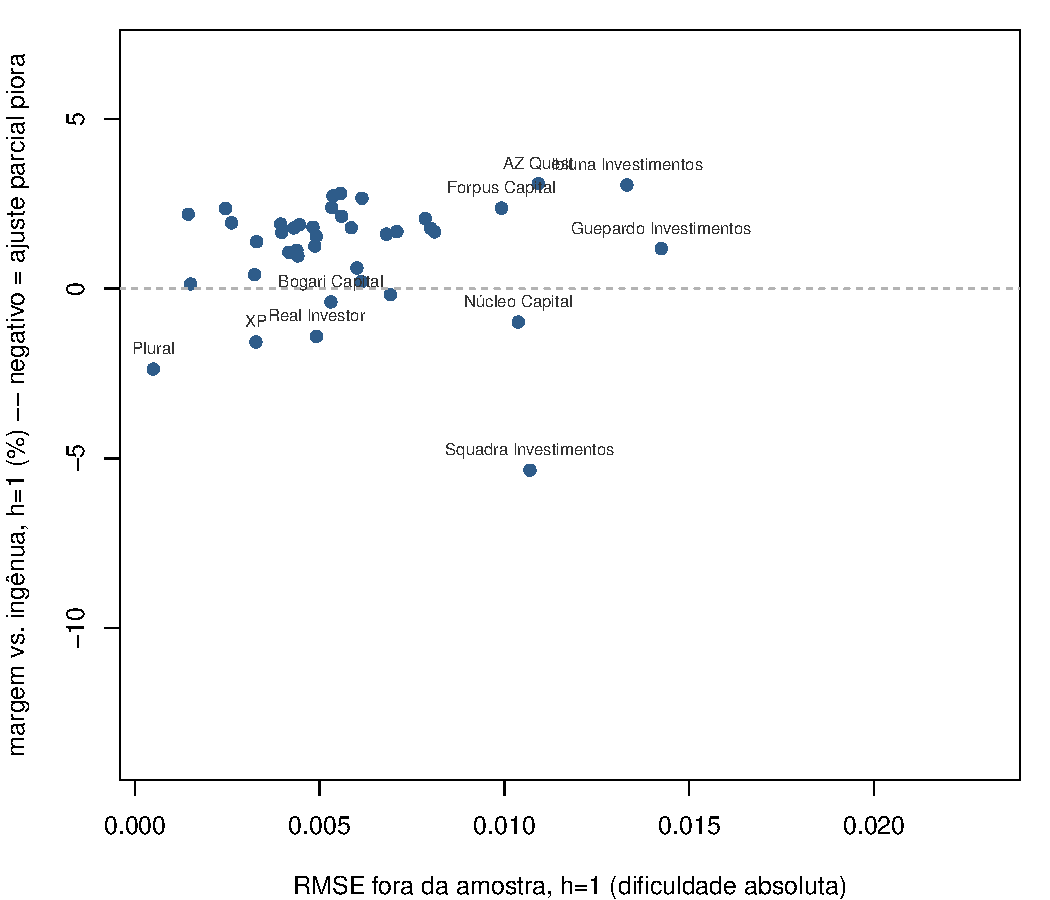
\includegraphics[width=0.7\textwidth]{fig_multihorizonte_gestora_rmse_margem.pdf}
\caption{Cada ponto é uma gestora: RMSE fora da amostra em $h{=}1$ (eixo $x$, dificuldade
absoluta) vs.\ margem sobre a ingênua em $h{=}1$ (eixo $y$, negativo = ajuste parcial piora).
Base: multiativo (2.347 fundos, 41 gestoras, 501 ativos).}
\end{figure}

% ======================================================================
\FloatBarrier
\section{Aplicação}
\label{sec:aplicacao}

\emph{[Seção ainda incerta quanto à inclusão no TCC, conforme indicação do orientador.
Descreve uma estratégia --- apelidada internamente de ``robô caça-replicantes'' --- que usa a
estrutura do erro fora da amostra (Seção~\ref{sec:resultados}) para identificar pares de fundos
cujo erro se move em sincronia além do que suas características observáveis explicam.]}

% ======================================================================
\FloatBarrier
\section{Conclusão}

\emph{[Seção a ser escrita após a Introdução.]}

\end{document}
